\documentclass[10pt,twoside,openright,titlepage]{ce}

% =Imports===============================================================================
\usepackage[]{tcolorbox}
\usepackage[]{amsmath,amssymb,amsthm}
\usepackage[]{graphicx}
\usepackage[]{color}
\usepackage[]{listings}
\usepackage[]{hyperref}
\usepackage[]{nielsformat}
\usepackage[]{subcaption}
\usepackage[]{tikz}
\usepackage[]{tikz-3dplot}
\usepackage[]{pgfplots}
\usepackage[]{pgfplotstable}

% =Definitions===========================================================================
\usepackage[]{nielstex}
\usepackage[]{nielstikz}

% Thesis specific definitions
\newcommand{\za}{\mathcal{A}}
\newcommand{\zb}{\mathcal{B}}
\newcommand{\zz}{\mathcal{Z}}

% For presenting the research questions, some stuff I stole of SO
% NOTE: not used as of now
\usepackage{enumitem}
\newlist{questions}{enumerate}{2}
\setlist[questions,1]{label=RQ\arabic*.,ref=RQ\arabic*}
\setlist[questions,2]{label=\thequestionsi.\arabic*,ref=\thequestionsi(\alph*)}

% =Document Attributes===================================================================
\msctitle{Sound Zones with a Cost Function based on Human Hearing}
\mscsubtitle{Subtitle Compulsory?}
\msckeywords{perceptual sound zones, sound field control, perceptual models, pressure matching}
\mscauthor{Niels Evert Marinus de Koeijer B.Sc.}
\msccity{Delft}
\msccountry{The Netherlands}
\mscnumber{??}
\mscdate{September 15, 2021}
\major{Electrical Engineering}
\mscinstitute{Delft University of Technology}
\mscfaculty{Electrical Engineering, Mathematics and Computer Science}
\mscdepartment{Microelectronics \& Computer Engineering}
\mscgroup{Circuits and Systems}
\chairperson{dr.ir. R.C. Hendriks}
\advisorone{dr. M. Bo M\o ller}
\advisortwo{dr. P. Martinez Nuevo}
\memberone{dr. M. Mastrangeli}
\membertwo{dr. J. Martinez Casta{\~n}eda }

% =Abstract==============================================================================
\def\ABSTRACT{\todo{Currently, this contains the draft of my thesis. 
Everything and anything can be changed as far as I'm concerned, I appreciate all feedback!}}

% =Document==============================================================================
\begin{document}

% =Front Pages===========================================================================
\frontmatter
\makecover
\maketitle
\makesignature
% Thesis Abstract ----------------------------------------------
%
\nonumchapter{Abstract}%
%
%
% The abstract you put in the preamble will appear here:
%
\ABSTRACT%
%
\cleardoublepage%

\nonumchapter{Acknowledgments}
\vskip 1cm
I would like to thank \FIRSTADVISOR, \SECONDMEMBER, \CHAIRPERSON, and \THIRDMEMBER\ for all their help and support during the project.
A special thanks to \SECONDMEMBER\ for often pushing me in the right direction through our numerous white board sessions.
Secondly, I would also like to especially thank \FIRSTADVISOR for being a major help during, and outside of the project.

In addition to this, I would like to thank Cassandra Gr\"utzner and especially 
Dorottya Hauk for their help proof reading the thesis 
and for many good times during the project.

\vskip 2cm
\noindent \AUTHOR \\
\PLACE \\
\DATE

\tableofcontents
% \listoffigures
% \listoftables
\mainmatter

% =Content===============================================================================
\chapter{Introduction}
\label{ch:introduction}
\section{Preface: the Sound Zone Problem}
\label{ch:introduction:preface}
Sound systems are used worldwide to fill rooms with enjoyable audio content. 
Problems arise however when multiple people in the same room want to enjoy different audio content at the same time.

For example, one person may want to enjoy a movie on the television, while others may want to listen to their music.
If they are in the same room, their desires clash: neither person can fully enjoy their chosen activity without disturbing
the other.
In short, the interference of multiple audio sources can lead to a situation where both individual experiences are diminished.

In recent years, attempts have been made to solve this problem by controlling the spatial reproduction of sound in such
a way that different areas in a room have distinct content, without interfering with each other.
This is typically done by controlling the sound pressure created by an array of loudspeakers.

One class of algorithms that attempt to do so are sound zone algorithms~\cite{betlehem2015personal}.
Sound zone algorithms partition the space of the room into multiple so-called sound zones.
Each sound zone is assigned different audio content.
The sound zone algorithms decide how to use the loudspeakers of the sound system to reproduce said audio content in every zone.
Using the principals of constructive and destructive interference, this is done in such a way that there is 
minimal interference between zones~\cite{betlehem2015personal}.
That is to say: the audio content of each zone is not audible in the others.

In the previously listed example, there would be one zone that would contain the audio of a movie and another zone that would contain music.
An image depicting the situation is given in \autoref{fig:introduction:motivation:concept}.
The sound zone algorithm determines how to best use the sound system to reproduce these two zones.
In the ideal case, both people can now enjoy the full potential of their audio content, without bothering one another.

\begin{figure}[]
    \centering
    \scalebox{1.0}{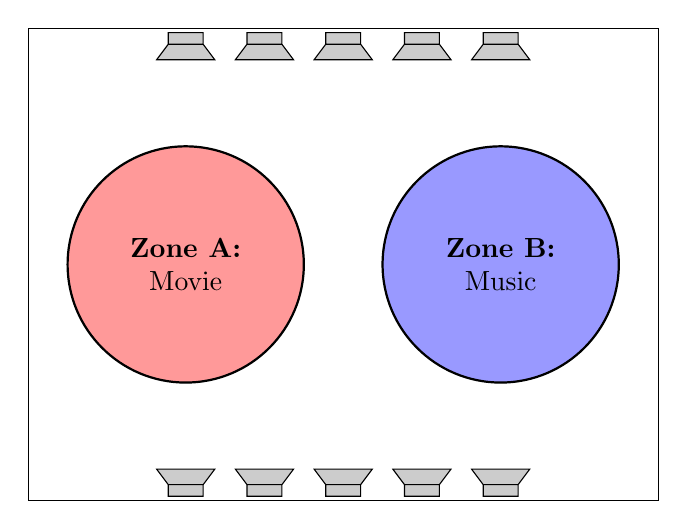
\begin{tikzpicture}
    \tikzset{
      Speaker/.pic={
        \filldraw[fill=gray!40,pic actions] 
        (-15pt,0) -- 
          coordinate[midway] (-front) 
        (15pt,0) -- 
        ++([shift={(-6pt,8pt)}]0pt,0pt) coordinate (aux1) -- 
        ++(-18pt,0) coordinate (aux2) 
        -- cycle 
        (aux1) -- ++(0,6pt) -- coordinate[midway] (-back) ++(-18pt,0) -- (aux2);
      }
    }

    \draw [draw=black] (0,0) rectangle (8,6);

    % Speakers on the top wall
    \pic[scale=0.7] at (2, 5.6) {Speaker};
    \pic[scale=0.7] at (3, 5.6) {Speaker};
    \pic[scale=0.7] at (4, 5.6) {Speaker};
    \pic[scale=0.7] at (5, 5.6) {Speaker};
    \pic[scale=0.7] at (6, 5.6) {Speaker};

    % Speakers on the bottom wall
    \pic[rotate=180, scale=0.7] at (2, 0.4) {Speaker};
    \pic[rotate=180, scale=0.7] at (3, 0.4) {Speaker};
    \pic[rotate=180, scale=0.7] at (4, 0.4) {Speaker};
    \pic[rotate=180, scale=0.7] at (5, 0.4) {Speaker};
    \pic[rotate=180, scale=0.7] at (6, 0.4) {Speaker};

    \draw[opacity=0.4, fill=blue] (6,3) circle[radius=1.5];
    \draw[thick] (6,3) circle (1.5) node[align=center] {\textbf{Zone B:}\\Music};
    \draw[opacity=0.4, fill=red]  (2,3) circle[radius=1.5];
    \draw[thick] (2,3) circle (1.5) node[align=center] {\textbf{Zone A:}\\Movie};
\end{tikzpicture}
}
    \caption{A room containing a sound system consisting of an array of loudspeakers and two zones.
                The goal of the sound zone algorithm is to control the sound system in such a way that the red zone
                contains the audio of a movie, and the blue zone contains the music.}
    \label{fig:introduction:motivation:concept}
\end{figure}

In practice however, the sound zone algorithm will not always do a perfect job~\cite{moller2016sound}.
The performance of algorithms depends on the environment and the available sound system.
Depending on the chosen zones, number and position of the loudspeakers, and the room, the interference between zones can typically only be reduced by so much.
As such, audio content of one zone is often still audible in other zones~\cite{moller2016sound}.

Improving sound zone algorithms is thus an active topic of research.
One recent approach is to include a model of the human auditory system, which models how sound is perceived by humans.
Typically, sound zone algorithms use sound pressure~\cite{betlehem2015personal}, which is a physical quantity characterizing the sound.
Sound pressure does not always accurately describe what is important for the perception of sound.
As such, including a perceptual model may allow the algorithm to focus on reproducing and canceling the parts of the audio content
that matter perceptually.

Early results show that a perceptual sound zone approach is promising.
Recent work by Donley et al. explored including the absolute threshold of hearing, which models the lowest sound pressure
humans can hear, into sound zone algorithms.
This pursuit found an increased quality of the reproduced audio in the zones~\cite{donley2015multizone}.
Other work by Lee et al. showed that including a perceptually-motivated weighting in the sound zone algorithm outperforms 
traditional algorithms~\cite{lee2019towards,lee2020signal}.

This work seeks to further explore this perceptual approach by proposing a novel perceptual sound zone algorithm and exploring
the benefits of including perceptual information.


\newpage
\section{Objectives and Organization}
\label{ch:introduction:objectives}
This section will state the goals of the thesis and organization of the rest of this document.
Als stated in the motivation, the goal of the thesis is to construct a perceptual sound zone algorithm.
The central question in this thesis is: 

{\centering\textit{``How can perceptual models of the human auditory system be used to improve sound zone algorithms?''}}

This question is answered in three steps. 
First, a perceptual model is selected in \autoref{ch:perceptual}.
Next, a sound zone algorithm is selected in \autoref{ch:sound_zone}.
Finally, the two are combined and the resulting algorithm is evaluated in \autoref{ch:perceptual_sound_zone}.
The organization of the three chapters is given below.

\subsection{Search and Implementation of a Perceptual Model}
\label{ch:introduction:objectives:perceptual}
In order to construct a perceptual sound zone algorithm, a perceptual model is required.
This begs the question: ``What perceptual models exist?''.
To answer this question, this chapter starts with a summary of necessary psycho-acoustics background in 
\autoref{ch:perceptual:background} followed by a literature review into state of the art perceptual models
in \autoref{ch:perceptual:review}.

To select a perceptual model suitable for combination with a sound zone algorithm, one must consider what 
desired properties of such a model.
These criteria and the resulting selection of one of the perceptual models from the 
literature review is given in \autoref{ch:perceptual:selection}.

The selected perceptual model is then discussed in greater detail in \autoref{ch:perceptual:implementation}. 
Here, implementation details are given and analysis are performed to give the reader an intuition into the model.

\subsection{Search and Implementation of a Sound Zone Approach}
\label{ch:introduction:objectives:sound_zone}
After selecting a perceptual model, a suitable sound zone approach must be selected.
Before determining which sound zone approaches are suitable, a literature review is performed in
\autoref{ch:sound_zone:approach_review} to document what sound zone approaches exist.

The perceptual model will impose certain constraints on which sound zone algorithm is best suited for integration.
As such, \autoref{ch:sound_zone:approach_selection} will reflect on these constraints to select one of the documented
sound zone approaches as the most promising for integration.

The sections that follow will discuss implementation details of the selected sound zone approach.
In \autoref{ch:sound_zone:data_model} a general sound zone data model will be given, formalizing the sound zone problem
and laying the mathematical foundation.
This mathematical foundation is then used in \autoref{ch:sound_zone:approach_implementation} and 
\autoref{ch:sound_zone:block_based} to derive a sound zone algorithm based on the selected sound zone approach.

The derived sound zone algorithm will form the foundation on which the perceptual sound zone algorithm will be built.
In addition to this, it will serve as a reference implementation with which the perceptual sound zone algorithm
can be compared.

\subsection{Implementation of a Perceptual Sound Zone Algorithm}
\label{ch:introduction:objectives:perceptual_sound_zone}


\chapter{Perceptual Model Review and Implementation}
\label{ch:perceptual}
\section{Introduction}
\label{ch:perceptual:introduction}
The goal of this chapter is to find a suitable perceptual algorithm for the creation of a perceptual sound zone algorithm.
This chapter is structured as follows.

The chapter will begin in \autoref{ch:perceptual:background} with some background information on the human auditory system.
This is done to ensure that the reader has the knowledge to understand the perceptual aspects of the thesis.

Next, with the necessary psycho-acoustical background in place, a literature review into perceptual models is given in \autoref{ch:perceptual:review}.
The purpose of this review is to document candidates for the perceptual model that will be used in the perceptual sound zone algorithm.
In addition to this, the reviewed models could also serve as potential candidates for use in the evaluation 
of the perceptual sound zone algorithm.

To perform the selection of a perceptual model from the candidates, criteria are be defined in \autoref{ch:perceptual:selection}. 
These criteria reflect desirable properties for a perceptual model to have for integration into sound zone algorithms.
The criteria are then used to make a selection.

Afterwards, the selected perceptual model is discussed in more detail in
\autoref{ch:perceptual:implementation} by stating implementation details and describing its behavior.
The chapter will then wrap up with some conclusions in \autoref{ch:perceptual:conclusion}.

\newpage
\section{Perceptual Background}
\label{ch:perceptual:background}
In the field of psycho-acoustics significant research has been done in characterizing the auditory 
perception and time-frequency
analysis capabilities of the human ear~\cite{painter2000perceptual}.
From this understanding, several perceptual models have been proposed which aim to model the 
perception of auditory stimuli by humans~\cite{van2005perceptual}.

Perceptual models are employed for various purposes.
Objective audio quality measures, for example, are perceptual models which aim to predict the perceived quality of audio~\cite{torcoli2021objective}.
In another example, perceptual audio coding uses models of auditory perception to minimize the perceived artifacts introduced when
performing the compression of audio~\cite{herre2019psychoacoustic}.

In general, many perceptual models operate on a time-frequency internal-ear representation of the input stimuli, obtained by applying an analysis filter bank. 
Among other effects, the filtering performed by the human ear is often taken 
into account at this stage~\cite{van2005perceptual, taal2012low}.
This representation is then used to determine its perceptually relevant aspects 
of the input stimuli~\cite{herre2019psychoacoustic}.

One aspect often used in perceptual models are the various auditory masking properties of the 
input stimuli~\cite{herre2019psychoacoustic}.
In general, auditory masking refers to the effects one sound has on the perception of other sounds~\cite{painter2000perceptual}.
In simultaneous masking, for example, one loud tone may overpower a tone of a similar frequency, rendering the 
latter tone inaudible~\cite{painter2000perceptual}.

Another aspect that is often used is the ``threshold of hearing'', which determines the minimum sound pressure level that can be perceived by a human~\cite{herre2019psychoacoustic}.
Combining this principle with the masking properties, one can define the ``masking threshold'' of input stimuli.
This threshold determines the sound pressure level required for other stimuli to be audible to a human observer in the presence of the input stimuli~\cite{painter2000perceptual} and is often used in perceptual 
models~\cite{van2005perceptual, taal2012low}. 
For example, the threshold of hearing is used in perceptual audio coding to 
make the coding artifacts inaudible~\cite{herre2019psychoacoustic}.

This chapter will motivate the use of the ``Par distortion detectability'' as the perceptual model used in perceptual sound zone algorithm framework proposed in \autoref{ch:sound_zone}, which is subsequently used in \autoref{ch:perceptual_sound_zone} to propose two perceptual sound zone algorithms.
In doing so, several other perceptual measures are discussed in detail, some of which are used in \autoref{ch:results} to evaluate the performance of the proposed algorithms.

The structure of this chapter is given as follows.
\begin{itemize}
    \item This chapter begins with \autoref{ch:perceptual:review} which documents a review of 
        possible candidate perceptual models from literature for use in the perceptual sound zone framework. 
    \item Next, \autoref{ch:perceptual:selection} motivates the selection of one of the reviewed candidates, 
        namely the ``Par distortion detectability'', as the perceptual model for use in the 
        proposed perceptual sound zone framework.
    \item Finally, the implementation and behavior of the ``Par distortion detectability'' is discussed in more detail in 
        \autoref{ch:perceptual:implementation}.
\end{itemize}

\newpage
\section{Review of Perceptual Models}
\label{ch:perceptual:review}
This section documents a literature review into perceptual models of the human auditory system.
This review is used in \autoref{ch:perceptual:selection} to determine which perceptual model is most 
suitable for use in a perceptual sound zone algorithm.

Especially promising are models that attach some ``score'' or ``rating'' to the perceptual quality of input signals.
These ratings can be used in algorithms to obtain an optimal rating through optimization.
In addition to this, they can also be used to quantify the quality of results from later algorithms.

As such, the focus of the literature review is not on the latest findings in the field of psycho-acoustics, or models 
that most accurately emulate the behavior of the human ear, but rather on algorithms that quantify quality.

To this end, in this section, two categories of perceptual models are considered.
First in \autoref{ch:perceptual:review:objective}, ``objective measures'' are discussed.
These are models which attempt to predict the perceptual quality ratings from listening tests. 
Next, perceptual models from ``audio coding'' are discussed in \autoref{ch:perceptual:review:audio_coding}.
These models are used to quantify how audible the artifacts of audio compression are.

\subsection{Review of Objective Measures}
\label{ch:perceptual:review:objective}
In order to objectively determine the perceived quality of audio one approach is to use listening tests.
These are tests in which subjects are asked to rate a property (or properties) of a set of audio stimuli.
One example where listening tests are used is for the evaluation of speech intelligibility of hearing aids~\cite{taal2011algorithm}.
Another example is determining which loudspeaker has higher perceived sound quality.

Performing listening tests is however often cumbersome due to the large amount of human labour involved.
This motivates the use of objective quality measures, which attempt to predict the outcomes of these objective listening tests.
This is very useful for algorithm developers, as they can get an indication of how well they are doing
without having to perform a labour intensive listening test~\cite{taal2011algorithm}.

Note however that a objective quality measure does not replace a listening test: it can only be used to give an 
indication.
Findings should always be confirmed with listening tests.

The objective measures that are considered in this review take a reference and degraded audio stimuli as inputs.
Most of the discussed models take the following approach.
First, input stimuli are converted to their so-called internal representations, which models how the 
human auditory system transforms the stimuli.
Various features are then derived from this internal representation.
The features are then mapped to a prediction of the results of a listening test.

These objective quality measures are promising for integration into sound zone algorithms as they summarize the 
quality of a signal into a single value, which can be potentially optimized for. 
It stands to reason that if an objective quality measure correlates with audio quality, optimizing over such a measure
could improve the sound quality of sound zone algorithms.

As such, this section explores various objective measures.
This is done by considering three classes different objective measures, namely: measures that quantify the quality 
and intelligibility of speech audio and measures for the general quality of audio. 

\subsubsection{Review of Objective Speech Quality Measures}
There have been a number of attempts to create objective measures to quantify the perceived quality of speech.
In this section three objective speech quality measures are discussed.
Namely the Perceptual Evaluation of Speech Quality (PESQ)~\cite{rix2001perceptual} measure,
Perceptual Objective Listening Quality Assessment (POLQA)~\cite{beerends2013perceptual}. measure, and 
Virtual Speech Quality Objective Listener (ViSQOL)~\cite{hines2012visqol,chinen2020visqol} measure.

\begin{itemize}
    \item 
    PESQ is a metric which attempts to determine the perceived quality of speech.
    It was standardized by the International Telecommunication Union (ITU-T) in 2001.
    PESQ is computed by first applying an auditory transform that maps the reference and degraded speech into a 
    time-frequency representation that models the perceived loudness of the signals.
    From this internal representation, so-called symmetric and asymmetric disturbances are determined 
    by computing differences between the time-frequency bins of the reference and degraded speech. 
    A non-linear average is then taken to obtain the average disturbance per time bin.
    These averaged disturbances are then mapped to the outcomes of listening test outcomes through linear 
    combination~\cite{rix2001perceptual}.

    \item
    POLQA is speech quality metric which was standardized by the International Telecommunication Union (ITU-T) in 2011. 
    It was intended to be the successor of PESQ, with the improvement of having more accurate predictions on a 
    wider range of distortions.
    POLQA works with a similar internal representation to PESQ, but computes distortion in a different way 
    as to be capable of handing global temporal compression and expansions~\cite{beerends2013perceptual}.

    \item
    ViSQOL is a metric developed in 2012 in a collaboration between Trinity College and Google.
    ViSQOL uses a different internal representation than PESQ and POLQA as it uses neurograms rather than loudness representations. 
    Neurograms contain the neural firing activity of the auditory nerve in time-frequency bins, and NSIM determines how similar
    the firing patterns of two neurograms are.
    The neurograms are then compared by means of the Neurogram Similarly Index Measure (NSIM).
    This similarity is then related to the outcomes of listening tests through a laplacian fit~\cite{hines2012visqol}, which is then used to make predictions.
\end{itemize}
In general, PESQ, POLQA and ViSQOL require many steps to compute and were found difficult to optimize for due to 
conditional branches within the algorithms and many non-differentiable steps such as clipping~\cite{rix2001perceptual,beerends2013perceptual,hines2012visqol}. 
Some attempts have been made however to reformulate PESQ in order to make it more tractable for optimization 
by approximating the disturbances by other functions~\cite{kim2019end}.

\subsubsection{Review of Objective Speech Intelligibility Measures}
Intelligibility of speech is defined as the percentage of words identified correctly given a degraded speech signal.
Objective speech intelligibility metrics seek to predict this percentage.
In this section, two of these metrics are discussed.
Namely, the Short Time Objective Intelligibility (STOI)~\cite{taal2011algorithm} measure and the 
Speech Intelligibility In Bits (SIIB)~\cite{van2017instrumental} measure.

\begin{itemize}
    \item 
    STOI was proposed by Taal et al. in 2011 as a speech intelligibility metric that could make accurate predictions 
    for a speech signals that were degraded time-frequency weighted distortions.

    For its internal representation, it finds a time-frequency internal representation through filtering the input stimuli with a filter bank consisting of 
    $1/3$ octave bands, and then segmented the filter taps into short time frames.
    Silent bins that do not contain speech are removed, and clipping is applied to limit the effect of one severely degraded time-frequency bin.
    The average correlation coefficient between the time-frequency bins of the internal representation of the reference and degraded 
    segments is then computed, and averaged over all bins to determine the intelligibility~\cite{taal2011algorithm}.
    \item 
    SIIB was introduced by Van Kuyk et al. in 2017 as a speech intelligibility metric that could be motivated through
    information theory through the mutual information rate.
    As such, SIIB is given in bits

    The idea behind SIIB is that the intelligibility of speech is related to the information shared between 
    intended and degraded speech.
    SIIB models how transformation of the reference speech signal to the degraded speech signal as a transmission channel.
    Among other aspects, this transmission channel includes a model of the human auditory system~\cite{van2017instrumental}.
    This communication channel is then used to compute the mutual information rate.
\end{itemize}

Both STOI and SIIB are difficult to optimize for directly. 

In STOI, the removal of silent regions and the clipping operator are non-differentiable operations.
Furthermore, the computation of the correlation coefficient is a non-convex function of the degraded speech~\cite{taal2011algorithm}.

SIIB is in general non-convex and non-differentiable as it uses the Karhunen-Lo\`eve transform and a 
K-nearest neighbor estimator to compute the mutual information rate.
However, if the communication channel is approximated as gaussian, the mutual information can be computed in closed form,
and SIIB becomes a differentiable measure~\cite{van2017instrumental}.

\subsubsection{Review of Objective Audio Quality Measures}
The previous objective quality metrics are both intended for evaluating speech.
In this section, a number of objective quality metrics are discussed that are designed instead 
for evaluating the perceived quality of general audio .
Namely, the Perceptual Evaluation of Audio Quality (PEAQ)~\cite{thiede2000peaq} 
and ViSQOLAudio~\cite{hines2015visqolaudio}.
The latter is an adapted version of the ViSQOL speech quality measures.

\begin{itemize}
    \item 
PEAQ is a audio quality metric standardized by the International Telecommunication Union (ITU-T).
PEAQ estimates a quality grade by first computing an internal representation  of
the reference and degraded audio signals.
This results in a time-frequency representation of the input stimuli from which a number of perceptually relevant feature,
referred to by PEAQ as Model Output Variables (MOVs), are extracted.
An example of these MOVs are the loudness of the noise or the bandwidth of the input stimuli.
These MOVs are then mapped to the final audio quality grade through a neural network~\cite{thiede2000peaq}.
    \item 
In 2015, it was found that with some adjustments ViSQOL could be used to determine audio quality, which resulted in a 
new metric ViSQOLAudio.
Among the adjustments were the removal of the voice activity detector included in ViSQOL and the use of a larger bandwidth
to cover the entire spectrum of hearing from 50 Hz to 20000 Hz, rather than just the bandwidth of speech~\cite{hines2015visqolaudio}.
\end{itemize}

PEAQ, and ViSQOLAudio are both difficult to optimize for.
A number of the MOVs computed in PEAQ, such as the partial noise loudness, are non-differentiable~\cite{thiede2000peaq}.
As ViSQOLAudio is similar to ViSQOL with some small adjustments, it is similarly difficult to optimize for~\cite{hines2015visqolaudio}.

\subsubsection{Review of Distraction Model}
One especially promising objective measure is the distraction proposed by Francombe et al. in 2015~\cite{francombe2015model}.
This measure was designed with the application of sound zones in mind.

The distraction was determined to be the keyword that best describes the perceptual experience of 
interfering audio programs.
This was determined through an elicitation study performed also performed by Francombe et al. 
in 2014~\cite{francombe2014elicitation}.
This prompted the creation of the model.

To create the model, a listening test was performed where the participants were subjected to audio-on-audio interference.
The subjects were played a target audio stimuli they were instructed to focus listening to.
At the same time, an interferer audio stimuli was played to distract the participant from the target.
The participants were given a scale between 0 and 100 on which they were asked to rate how distracting the interference
was when listening to the target program, where a 100 indicates that the interferer ``overpowered'' the target audio~\cite{francombe2015model}.

The target-interferer stimuli pairs and corresponding ratings resulted in a dataset.
This dataset was then used to fit a model which predicted the distraction given novel a target-interferer stimuli pair.
The model consisted of taking a linear combination of 5 features that were computed from the stimuli~\cite{francombe2015model}.

Computing said features could however not be performed in real time.
The reason for this was that as the original distraction model is too computationally complex~\cite{ramo2017real}.
To this end, in 2017, R\"am\"o et al. proposed a version of the distraction model that could be run in real-time.
This was done by approximating the features of the original distraction model by computationally less complex alternatives.
The resulting real-time distraction model was found to be less precise, but could be run in 0.04\% of the time of the 
original distraction model~\cite{ramo2017real}.

On face value, the real-time distraction model seems promising to optimize over.
However, while easy to compute, the model is non-differentiable as the model uses
piecewise functions and non-convex due to taking the logarithm of the square of the input signals.
In addition to this, the model also performs operations that are difficult to express mathematically, such as counting 
the number of short-time blocks that exceed a certain threshold~\cite{ramo2017real}.

\subsection{Review of Perceptual Models used in Audio Coding}
\label{ch:perceptual:review:audio_coding}
The second class of perceptual models that are considered are the perceptual models used in audio coding.
Audio coding algorithms attempt to find an low-bitrate representation of an audio input signal, which is a 
form of lossy compression.
As such, audio coding algorithms typically introduces errors in doing so, which can be a detriment to the listening experience.

To minimize the impact of these errors, 
many audio coding algorithms use a perceptual model to quantify how disturbing the introduced distortions are.
The perceptual model is used to introduce encoding errors in such a way that the audio output
signal is perceptually indistinguishable from the audio input signal~\cite{taal2012low}.
This model typically takes form of a distortion function which determines how
audible the difference between a reference input audio signal and a distorted output audio signal is.
This function can used to for example encode an input audio signal such that it has minimal distortion for a
specified bitrate.

The perceptual models used in audio coding are promising for integration into a sound zone algorithm, as they are 
often mathematically tractable.
As stated, these perceptual models typically take the form of some sort of distortion function that quantifies
how perceptually disturbing the introduced artifacts are. 
One approach for example could be to define sound zone algorithms that minimize a distortion function.

As such this section explores three perceptual models from audio coding.

\subsubsection{Review of Perceptual Models from ISO MPEG Standard}
The ISO/IEC 11172-3 standard specifies a coded representation for audio files~\cite{ISO11172-3}, 
and a corresponding decoder.
An encoder said representation is not part of the standard.
This is done deliberately, to allow for future improvements to the encoder, without having to change the standard~\cite{pan1995tutorial}.

The standard does however provide a number of examples of possible encoders, with increasing complexity.
Alongside these example encoders, two psycho-acoustical models are included for use during the encoding process. 

The psycho-acoustical models work by subdividing the input audio signal into frequency bands which correspond to the 
frequency bands in the human auditory system.
The model then determines how much quantization noise can be added separately per band without the noise becoming audible.
As such, the model assumes that the distortion signal is noise-like~\cite{van2005perceptual}, which is usually
the case for quantization noise for audio coders.

The output of the psycho-acoustical model is thus the amount of noise that can be added per band.
In the case of audio coding, this can then be used to control quantization noise.
Note that this perceptual model does not come in the form of the earlier described distortion function.
This technique has however been used for various signal processing purposes, 
such as audio watermarking~\cite{taal2012low}.
As such, examples exist from which optimization schemes could be inspired.

\subsubsection{Review of Par Detectability Measure}
In 2005, van der Par et al. proposed a novel perceptual model designed for use in audio coding~\cite{van2005perceptual}.
The model defines a distortion measure which determines the ``detectability'' of a distortion signal 
in presence of  masking signal.
That is to say, the function quantifies the degree to which a human is to detect a distortion signal.
For audio coding purposes, this distortion signal is error introduced due to the audio compression.

Similarly to the ISO MPEG perceptual models, the Par detectability typically operates on short-time segments, typically in the order of 20 to 200 milliseconds.
The proposed method however differentiates itself from the previously discussed ISO MPEG models in three ways.

Firstly, the paper uses newer findings from psycho-acoustic literature, namely spectral integration.
In spectral integration, the masking effects from neighboring bands are taken into account when computing the 
masking effects.
The psycho-acoustical models defined in the ISO MPEG standard does not do this as it effectively 
works independently per band~\cite{taal2012low}.

Secondly, it assumes that the distortion signal is sinusoidal, rather than noise-like.
As such, it is more effective in hiding sinusoidal distortion.

Thirdly and finally, the perceptual model is described as a distortion function which quantifies how 
detectable a disturbance stimuli is.
The proposed distortion measure can be expressed as a squared L2-norm.

This mathematical tractability makes for easy integration into existing least-square problems.
As such, the Par model has been used in many signal processing applications, 
examples ranging from speech enhancement to removing perceptually irrelevant sinusoidal 
components~\cite{balazs2009time, taal2013optimal}.

\subsubsection{Review of Taal Detectability Measure}
A paper from 2012 by Taal et al. proposed a novel perceptual model \cite{taal2012low} which introduces a
alternative definition to the detectability defined in the Par model.

In contrast to the Par detectability, the Taal detectability measure takes temporal characteristics of a signal into account.
The inclusion of temporal information allows for the suppression of ``pre-echoes'', which is an artifact that 
the Par model suffers from. 
The ``pre-echoes'' artifacts arises from the assumption that the masking effects of the masking signal are stationary across 
time. 
As a result, audio coding algorithms may assume that audio content is masked while it is not, which could results in quantization
noise not being masked.

In contrast to other temporal perceptual models, the Taal Detectability has a relatively low computational complexity.
In addition to this, it can also be expressed as a squared L2-norm.
The computational demand was however shown to be higher than the Par Detectability~\cite{taal2012low}, especially for longer time segments.

\newpage
\section{Selection of Perceptual Model}
\label{ch:perceptual:selection}
In \autoref{ch:perceptual:review} a literature review of various models of the human auditory system were given.
In this section, one perceptual model will be selected for use in a sound-zone algorithm.

The other perceptual models will still be of use however during the evaluation of the results of the perceptual
sound zone algorithm.

The approach to select a perceptual model is as follows.
First, \autoref{ch:perceptual:selection:criteria} will discuss the criteria that will inform the decision.
Next, \autoref{ch:perceptual:selection:selection} will use these criteria to evaluate the perceptual models
discussed in the literature review in \autoref{ch:perceptual:review}.
From this evaluation the most suited perceptual model will be selected for use in a perceptual sound zone 
algorithm.

\subsection{Criteria for Selecting Perceptual Model}
\label{ch:perceptual:selection:criteria}
This section will define desirable criteria for the perceptual model for integration with a sound zone algorithm.
These criteria will be used to select a perceptual model from the models discussed in the literature review.
\begin{enumerate}
    \item \textbf{Mathematical Tractability.}\\
        It is a desirable property for the perceptual model to be easy to include in optimization problems.
        For example, perceptual models that can are differentiable are therefore favoured over optimization problems
        that are non-differentiable.
    \item \textbf{Computational Overhead:}\\
        It is desirable for the inclusion of the perceptual model to add minimal computational load 
        to the sound zone algorithm.
        The additional overhead of the perceptual model should not increased the run time of the sound zone algorithm by many orders of magnitude.
\end{enumerate}

\subsection{Selection of Perceptual Model}
\label{ch:perceptual:selection:selection}
This section will use the criteria defined by \autoref{ch:perceptual:selection:criteria} in order to select a perceptual
model.
In the literature review given in \autoref{ch:perceptual:review}, two classes of perceptual model were considered:
perceptual models from audio coding and objective audio measures.

All objective audio measures were found to be mathematically untractable, as all models are both non-differentiable and 
non-convex functions of their input signals.
As such, they are difficult to integrate into existing sound zone algorithms.
However, as the objective audio measures predict the outcomes of listening tests, they are uniquely suited for evaluation
of the results.

All models from audio coding are mathematically tractable and of low computational overhead.
The ISO MPEG models were found to be less promising than the Par and Taal detectability as it does not immediately 
define a cost function which can be optimized over.
The ISO MPEG models only determines how much noise can be added per frequency band, but does not provide an immediate 
means of using that information in optimization.

As such, the decision is between the Par and Taal detectability.
As discussed, the Taal detectability takes into account more perceptual.
This is however this has been shown to be at the cost of computational complexity.
As such, the Par detectability will be selected for use in the sound zone algorithm.



\newpage
\section{Implementation of Selected Perceptual Model}
\label{ch:perceptual:implementation}
The Par distortion detectability is the perceptual model used in the proposed perceptual sound zone framework.
In this section, to give the reader a greater understanding of the model, the Par distortion detectability measure is considered in greater detail.

This section is organized as follows.
First, \autoref{ch:perceptual:implementation:intuition} gives a high-level description of the Par distortion detectability, providing an intuitive understanding and introducing some of the notation that is used.
Next, the steps for computing the distortion detectability are described in 
\autoref{ch:perceptual:implementation:computation}.
Finally, \autoref{ch:perceptual:implementation:least_squares} rewrites the distortion detectability into terms of a squared $L^2$-norm and provides some analysis of the behavior of the resulting representation.

\subsection{High-Level Description of the Par Distortion Detectability}
\label{ch:perceptual:implementation:intuition}
In this section, a high-level description of the Par distortion detectability measure is given.
This is done to give the reader a basic understanding of the model before going into greater detail.

The Par distortion detectability maps two input sequences to a positive real value, i.e. $D: (\Real{N_x}, \Real{N_x})\mapsto \Real{+}$.
The two input sequences are the masking signal $x[n]\in\Real{N_x}$ and the disturbance signal $\varepsilon[n]\in\Real{N_x}$.
The distortion detectability of these two sequences is denoted as $D(x[n], \varepsilon[n])$. 

Imagine a human listening to both the masking signal $x[n]$ and the disturbance signal $\varepsilon[n]$ simultaneously.
The distortion detectability $D(x[n], \varepsilon[n])$ can be understood as how easily a human listener can detect the disturbance signal $\varepsilon[n]$ in presence of the masking signal $x[n]$.
The signal $x[n]$ is referred to as the masking signal because its masking properties are used to determine how well it masks the disturbance signal $\varepsilon[n]$.

For this interpretation to be accurate, the signals $x[n]$ and $\varepsilon[n]$ should be short-time signals.
The paper uses a signal length of 20 to 200 milliseconds~\cite{van2005perceptual}.    
This is important, as the model assumes that the psycho-acoustical properties of $x[n]$ and $\varepsilon[n]$ are stationary.  

The measure is normalized in such a way that the distortion detectability $D(x[n],\varepsilon[n])$ is equal to 1 when the disturbance signal $\varepsilon[n]$ is ``just noticeable'' in presence of masking signal $x[n]$.
That is to say: if the distortion detectability is 1, the disturbance is on the verge of being noticeable and not noticeable.

The distortion detectability $D(x[n],\varepsilon[n])$ can also attain a value larger than $1$.
The larger values of the distortion detectability correspond with an increased perceived presence of the disturbance signal $\varepsilon[n]$.

\subsection{Computation Details of the Par Distortion Detectability}
\label{ch:perceptual:implementation:computation}
This section explores calculating the Par distortion detectability.k
The first thing to note about the Par distortion detectability is that it is computed using the frequency domain representations of its inputs~\cite{van2005perceptual}. 
To this end, let $X[k]$ and $\mathcal{E}[k]$ denote the frequency domain representations of the masking signal $x[n]$ and 
the disturbance signal $\varepsilon[n]$ respectively.

After determining the frequency domain representations, 
the Par distortion detectability computes an internal representation of the input signals $X[k]$ and $\mathcal{E}[k]$.
This internal representation models how the input stimuli appear to the human auditory system.
For the Par distortion detectability measure, this is modeled by filtering the input stimuli.

Two subsequent filters are applied.
The first filter models how parts of the ear filter the incoming sound with an outer- and middle-ear filter $H_\text{om}[k]$. 
Next, a $4^\text{th}$ order Gammatone filter bank is applied, modeling the frequency-place transform that occurs in 
basilar membrane inside of the ear~\cite{van2005perceptual}.

The Gammatone filter bank consists of $N_g$ filters.
The frequency-domain representation of each individual filter is denoted by $\Gamma_i[k]$, for $1 \leq i \leq N_g$. 
The filters in the filter bank $\Gamma_i[k]$ have a bandwidth given by the equivalent 
rectangular bandwidth (ERB) and center frequencies are given by the corresponding equivalent rectangular bandwidth number
scale (ERBS).
Expressions for the gammatone filters $\Gamma_i[k]$ are provided by the original paper~\cite{van2005perceptual}.

After filtering, the power per Gammatone filter tap is computed.
Let $M_i$ and $S_i$ denote the output power of the $i^\text{th}$ filter tap for the masking signal $X[k]$ and 
the disturbance signal $\mathcal{E}[k]$ respectively.
This output power can be understood as the amount of power perceived per frequency band of the human ear. 
The relationship between the input quantities and the output power of the filter taps can be given as follows:
\begin{align}
    M_i &= \frac{1}{N_x}\sum_{k=0}^{N_x-1}\left|H_\text{om}[k]\right|^2\left|\Gamma_i[k]\right|^2\left|X[k]\right|^2, \\
    S_i &= \frac{1}{N_x}\sum_{k=0}^{N_x-1}\left|H_\text{om}[k]\right|^2\left|\Gamma_i[k]\right|^2\left|\mathcal{E}[k]\right|^2. 
\end{align}
The output powers can then be used to define the within-channel distortion detectability $D_i$ per filter tap $i$.
This can be thought of the distortion detectability per frequency band of the human ear, and is defined as follows:
\begin{align}
    D_i = \frac{N_xS_i}{N_xM_i + C_a}.
\end{align}
Here, $C_a$ is a calibration constant that ensures that the absolute threshold of hearing is predicted correctly.
This can be understood by considering the case where no masking signal $x[n]$ is present, 
in which case $M_i = 0$ for all $i$.
If not for the calibration constant $C_a$, the distortion detectability of any non-zero disturbance
$\varepsilon[n]$ would be infinite.
In order to take the frequency-dependence of the threshold of hearing into account, the previously described outer- and middle ear filters are defined as the inverse of the threshold of hearing~\cite{van2005perceptual}.

The distortion detectability $D(x[n],\varepsilon[n])$ can then be computed as the scaled sum of all 
within channel distortion detectabilities.
It is defined as follows:
\begin{align}
    D(x[n],\varepsilon[n]) &= C_s L_\text{eff}\sum_{i=0}^{N_g} D_i \\
                        &= C_s L_\text{eff}\sum_{i=0}^{N_g} 
                        \frac{\sum_{k=0}^{N_x-1}\left|H_\text{om}[k]\right|^2\left|
                            \Gamma_i[k]\right|^2\left|\mathcal{E}[k]\right|^2}
                        {\sum_{k=0}^{N_x-1}\left|H_\text{om}[k]\right|^2\left|
                            \Gamma_i[k]\right|^2\left|X[k]\right|^2 + C_a}.
    \label{eq:perceptual:implementation:computation:detectability}
\end{align}
Here, $C_s$ is a calibration constant chosen such that a just noticeable disturbance signal results in a 
detectability of $D(x[n],\varepsilon[n]) = 1$. 
The constant $L_\text{eff}$ is the integration time of the human auditory system.
It is chosen equal to the segment length of $x[n]$ and $\varepsilon[n]$ in milliseconds.  

In order to further understand distortion detectability, consider the behavior of the expression of the 
detectability $D(x[n],\varepsilon[n])$ above.
Imagine that the spectrum of the masking signal is much larger than the disturbance signal, 
i.e. $X[k] \gg \mathcal{E}[k]$ for all frequency bins $k$.
In this case, the detectability of $\varepsilon[n]$ will be small due to the masking of the masking signal $x[n]$ or
due to the threshold of hearing (determined by the calibration constant $C_a$).

Conversely, consider the case that the spectrum of the masking signal is much smaller than the disturbance signal,
i.e. $X[k] \ll \mathcal{E}[k]$ for all frequency bins $k$.
In this case, the resulting detectability is determined greatly by the calibration coefficient~$C_a$: 
\begin{itemize}
    \item If the total energy of the filtered disturbance signal is much larger than the calibration constant 
        $S_i \gg C_a$ for all $i$, the distortion detectability becomes large.
        This models the case that the disturbance signal is large relative to the threshold of hearing.
    \item Alternatively, if $S_i \ll C_a$ for all $i$, the disturbance signal is inaudible due to the threshold of hearing, and the distortion detectability will be low accordingly.
\end{itemize}

The determination of the calibration constants $C_a$ and $C_s$ is discussed in \autoref{ch:perceptual:implementation:calibration}.


\subsection{Least-Squares Formulation of the Par Distortion Detectability}
\label{ch:perceptual:implementation:least_squares}
This section will rewrite the previously introduced detectability into a least-squares representation~\cite{taal2012low}. 
This representation is more mathematically tractable than 
\autoref{eq:perceptual:implementation:computation:detectability} and thus 
will allow for easier integration into existing sound zone algorithms.

To obtain this expression, the sum of squares will be expressed as a $L^2$ norm.
Consider the following rewrite of the detectability given in 
\autoref{eq:perceptual:implementation:computation:detectability}: 
\begin{align*}
    D(x[n],\varepsilon[n]) &= C_s L_\text{eff}\sum_{i=0}^{N_g}
                        \frac{\sum_{k=0}^{N_x-1}\left|H_\text{om}[k]\right|^2\left|
                            \Gamma_i[k]\right|^2\left|\mathcal{E}[k]\right|^2}
                        {\sum_{k=0}^{N_x-1}\left|H_\text{om}[k]\right|^2\left|
                            \Gamma_i[k]\right|^2\left|X[k]\right|^2 + C_a} \\
                           &= \sum_{i=0}^{N_g}
                           \left(\frac{C_s L_\text{eff}}{\norm[2][2]{H_\text{om}[k]\Gamma_i[k]X[k]} + C_a}\right)
                        \sum_{k=0}^{N_x-1}\left|H_\text{om}[k]\right|^2\left|
                        \Gamma_i[k]\right|^2\left|\mathcal{E}[k]\right|^2 \\
                           &= \sum_{k=0}^{N_x-1}\left(\sum_{i=0}^{N_g}
                            \frac{C_s L_\text{eff}\left|\Gamma_i[k]\right|^2}
                                 {\norm[2][2]{H_\text{om}[k]\Gamma_i[k]X[k]} + C_a}\right)
                        \left|H_\text{om}[k]\right|^2\left|\mathcal{E}[k]\right|^2 \\
                           &= \sum_{k=0}^{N_x-1}\left|W_x[k]\right|^2\left|\mathcal{E}[k]\right|^2 \\
                           &= \norm[2][2]{W_x[k]\mathcal{E}[k]}. 
\end{align*}
In this case, the norm is taken over the frequency-domain sequence indexed by $k$.
The rewrite above introduced perceptual weighting $W_x[k]\in\Real{N_x}$ informed by the auditory masking effects of the masking signal $x[n]$. 
The entries of the perceptual weighting can be understood as the importance of those frequencies for the total detectability.
The perceptual weighting $W_x[k]$ is defined as follows: 
\begin{equation}
    W_x[k] = \left(\sqrt{\sum_{i=0}^{N_g}\frac{C_s L_\text{eff}\left|\Gamma_i[k]\right|^2}
        {\norm[2][2]{H_\text{om}[k]\Gamma_i[k]X[k]} + C_a}}\right)
        \left|H_\text{om}[k]\right|.
\end{equation}
Note from this formulation that the perceptual weighting is only a function of the masking signal $x[n]$.

Note also that the resulting detectability $D(x[n],\varepsilon[n])$ is a convex function 
of the disturbance signal $\varepsilon[n]$. 
This can be seen as follows.
The frequency-domain representation $\mathcal{E}[k]$ is related to the 
time-domain representation $\varepsilon[n]$ through the DFT, which is a linear operator.
The perceptual weighting of $\mathcal{E}[k]$ performed by $W_x[k]$ is also a linear operation.
As such, $W_x[k]\mathcal{E}[k]$ is an affine function of $\varepsilon[n]$.
Finally, as the composition of an affine mapping and a convex function is convex~\cite{boyd2004convex},
the Par detectability distortion
is convex in $\varepsilon[n]$.

In order to gain a deeper understanding of the behavior of the perceptual weighting $W_x[k]$, consider 
\autoref{fig:perceptual:implementation:least_squares:masking_expl}.
The figure relates the auditory masking threshold and the corresponding perceptual weighting when a 1000 Hz tone at 70 dB SPL is used as masking signal $x[n]$.
The top plot depicts the masking threshold, and the bottom plot depicts the corresponding perceptual weighting.

Recall that the masking threshold is the minimal sound pressure level that is required for an additional stimulus to be audible in the presence of the masking signal~\cite{painter2000perceptual}.
In addition to this, the threshold of hearing is also depicted to highlight the additional masking that occurs due to the masking signal.

As can be seen, the masking threshold peaks at 52 dB SPL at 1000 Hz.
This implies that a different tone at the same frequency must be at least 52 dB SPL to be audible.
As depicted, this results in a low perceptual weighting at 1000 Hz, implying that a disturbance at this frequency is less detectable.
Note also that the low and higher frequencies are also weighted lower due to the threshold of hearing.
This implies that these frequencies are less important perceptually.

\begin{figure}[]
    \centering
    \scalebox{1.0}{\begin{tikzpicture}
    \begin{groupplot}[group style={group size=1 by 2, vertical sep=2cm}, xmajorgrids=true, ymajorgrids=true]
        \nextgroupplot[xmode=log, xlabel={Frequency [Hz]}, ylabel={Pressure [dB SPL]}, ylabel near ticks, 
            title={Masking Threshold for a 1 KHz sine at 70 dB SPL}, scale only axis, 
            height=3cm, width=9cm, xmin=10, xmax=20000, ymin=-20, ymax=120]
        %xmin=5000, xmax=6400, xtick={5000, 5200, 5400, 5600, 5800, 6000, 6200, 6400},
        %ymin=-0.5, ymax=0.5]
        \addplot [color=red, dashed]
        table [x expr=\thisrow{fr}, y expr=(\thisrow{tq}), col sep=comma] 
            {data/masking.csv};
        \addplot [color=red]
        table [x expr=\thisrow{fr}, y expr=(\thisrow{tx}), col sep=comma] 
            {data/masking.csv};
        \addplot [color=black]
        table [x expr=\thisrow{fr}, y expr=(\thisrow{x}), col sep=comma] 
            {data/masking.csv};

        \nextgroupplot[xmode=log, xlabel={Frequency [Hz]}, ylabel={Weight}, ylabel near ticks, 
            title={Par Detectability Perceptual Weighting for a 1 KHz sine at 70 dB SPL}, scale only axis, 
            height=3cm, width=9cm, xmin=10, xmax=20000, ymin=0, ymax=50]
        %xmin=5000, xmax=6400, xtick={5000, 5200, 5400, 5600, 5800, 6000, 6200, 6400},
        %ymin=-0.5, ymax=0.5]
        \addplot [color=red, dashed]
        table [x expr=\thisrow{fr}, y expr=(\thisrow{dq}), col sep=comma] 
            {data/masking.csv};
        \addplot [color=red]
        table [x expr=\thisrow{fr}, y expr=(\thisrow{dx}), col sep=comma] 
            {data/masking.csv};
    \end{groupplot}
\end{tikzpicture}
}
    \caption{Depiction of the masking threshold and corresponding perceptual weighting 
        function for a 1000 Hz tone with an amplitude of 70 dB SPL.
        The threshold of hearing is also depicted.}
    \label{fig:perceptual:implementation:least_squares:masking_expl}
\end{figure}

\newpage
\section{Conclusion}
\label{ch:perceptual:conclusion}
The goal of this chapter was to determine a suitable perceptual model for integration into a sound zone algorithm.
This was done by first reviewing various objective quality measures and perceptual models from audio coding.

To select a suitable model, the mathematical tractability and the additional computational overhead of each model under
review was considered.
From this, it was found that the Par detectability was found to be the most promising perceptual model included in the
review.
Finally, the chapter concluded with an analysis and implementation of the Par detectability.



\chapter{Sound Zone Approach Review and Implementation}
\label{ch:sound_zone}
\section{Introduction}
\label{ch:sound_zone:introduction}
The goal of this chapter is find a suitable sound zone approach for integration with the perceptual model selected in \autoref{ch:perceptual}.

The chapter will start with \autoref{ch:sound_zone:approach_review} which will provide a review of various sound zone approaches from literature to provide a selection to choose 
from.

After documenting the state of the art, one sound zone algorithm will be selected in \autoref{ch:sound_zone:approach_selection} as the most promising 
for combination with the perceptual model selected in \autoref{ch:perceptual}.
This is done by reflecting on the mathematical properties of the selected perceptual model.

After selecting a sound zone approach, the rest of the chapter will focus on the derivation and the implementation of a sound zone algorithm that takes 
said approach.
This algorithm will serve two purposes.
Firstly, it will serve as the basis upon which the perceptual sound zone algorithm will be built.
Secondly, it is well suited as a reference with which the perceptual sound zone algorithm can be compared.

To derive said sound zone algorithm, \autoref{ch:sound_zone:data_model} will start by introducing the data model.
This is followed by the implementation of the selected algorithm in \autoref{ch:sound_zone:approach_implementation}.
The implementation is then extended in \autoref{ch:sound_zone:block_based} to operate in a short-time block-based fashion, 
giving the algorithm the potential to run in real-time.
The chapter ends with a summary and concluding remarks in \autoref{ch:sound_zone:conclusion}.

\newpage
\section{Description of Sound Zone Problem}
\label{ch:sound_zone:problem}
An initial description of the sound zone problem was given in the introduction of the thesis.
This section seeks to build on this description in order to provide the understanding necessary 
for the rest of this work.

As mentioned in the introduction, the problem that sound zones seeks to solve is the reproduction
of multiple types of audio content in the same room with minimal interference.
This way, multiple people can enjoy different audio content without disturbing one another.

Controlling the spatial distribution of sound is done by controlling the 
audio that is produced by an array of loudspeakers.
The space inside the enclosure is divided up into multiple zones.
Each zone is assigned target sound pressure that we would like to have reproduced inside of it.
This target sound pressure could be various audio content, for example music or the sound of a movie.

To understand this principal, consider the example given by \autoref{fig:sound_zones:background:content}.
The loudspeakers array that is present in the room is to be controlled by the sound zone algorithm 
in such a way that the desired content is reproduced in each zone.
As mentioned, this is to be done in a way that results in minimal interference, e.g. it is undesirable
to be able to hear content B when inside the red zone.

\begin{figure}[h]
    \centering
    \scalebox{1.0}{\input{tikz/tikz_2D_room_concept_content.tex}}
    \caption{A birds-eye view of a room is depicted.
        It is divided into two zones: a red zone and a blue zone.
        Each zone is assigned different content: content A and content B.
        In the northern and southern parts of the room, a loudspeaker array is mounted on the walls.
        }
    \label{fig:sound_zones:background:content}
\end{figure}

There are various approaches to solving the sound zone problem.
An important concept that is used frequently is that bright zones and dark zones.

Sound zone problems are typically decomposed into a separate subproblem for every zone.
Each one of these subproblems considers only two zones: one bright zone and one dark zone.
The goal of each subproblems is to reproduce a specified target sound pressure in the bright zone while restricting the 
sound pressure in the dark zones.

The combination of all subproblems provides a solution to the sound zone problem. 
To ease the understanding of this concept, consider an example of this decomposition is given in 
\autoref{fig:sound_zones:background:bright_dark_example}.

Here, a decomposition of the example given in \autoref{fig:sound_zones:background:content} into 
two bright-dark zone pairs.
For the first problem, the goal is to reproduce content A in bright zone A while minimizing 
the amount of sound pressure in dark zone A.
Similarly for the second problem: reproduce content B in bright zone B while minimizing the 
amount of sound pressure in dark zone B.
Combining the two solutions results in a solution with content reproduced in both zones with 
minimal interference between zones.

\begin{figure}[]
    \centering
    \begin{subfigure}{0.49\linewidth}
        \centering
        \scalebox{0.9}{\input{tikz/tikz_2D_room_concept_bright_dark_zone_A.tex}}
    \end{subfigure}
    \begin{subfigure}{0.49\linewidth}
        \centering
        \scalebox{0.9}{\input{tikz/tikz_2D_room_concept_bright_dark_zone_B.tex}}
    \end{subfigure}
    \caption{A birds-eye view of a room is depicted twice containing two different sound zone problems.}
    \label{fig:sound_zones:background:bright_dark_example}
\end{figure}

This concludes the introduction to the sound zone problem.
The goal of the rest of this chapter is find a suitable sound zone approach 
for integration with the perceptual model selected in \autoref{ch:perceptual}.

Before selecting an approach, a review of sound zone literature is given.
As such, the chapter will start with a brief description of sound zones in \autoref{ch:sound_zone:problem} to give the reader 
the necessary background information on the sound zone problem.
Afterwards, \autoref{ch:sound_zone:data_model} will present the mathematical framework  
used to describe the sound zone problem.

This mathematical framework is then used to describe the two main sound zone approaches, ``Pressure Matching'' and ``Acoustic Contrast Control'', 
in \autoref{ch:sound_zone:approaches}.
One of these approaches will be used in the perceptual sound zone algorithm.

In order to determine which one is most suited, \autoref{ch:sound_zone:approach_selection} will reflect on the mathematical 
properties of the 
Par detectability selected in \autoref{ch:perceptual}.
From this, one approach will be selected.

% \subsection{Sound Zone Approaches}
% \label{ch:sound_zone:problem:solutions}
% With the sound zone problem sufficiently explained, this section will now cover various sound zone approaches.
% These approaches describe a general manner of solving the sound zone problem.

% \subsubsection{Delay and Sum Beamforming}
% One traditional approach to creating sound zones is delay and sum (DS) beamforming~\cite{olik2013comparative}.
% In beamforming an array of loudspeakers is used to focus a ``beam'' of audio.
% This is done using the principals of constructive and destructive interference by playing with slight delays from each loudspeaker in the array (hence, 
% the name ``delay and sum'').
% The beam is constructed through constructive interference, whereas outside of the beam the audio content is partially canceled through destructive interference.

% For sound zone applications, the angle of the beam is chosen such that the target audio is directed towards its respective bright zone.
% Beamforming is somewhat limited for sound zone applications as it limits the spatial control to an angled beam.
% The other sound zone algorithms that will be discussed in this section can be considered a generalization of beamforming, as their framework supports more
% spatial control.

% \subsubsection{Pressure Matching Approach}
% In pressure matching approaches (PM), one attempts to control the output of the loudspeaker array in such a way that resulting sound pressure in the zone 
% matches the specified target sound pressure for that zone.
% While doing so, the PM approach attempts to minimize the sound pressure that results in other zones as to minimize the interference or crosstalk between zones
% ~\cite{olik2013comparative, betlehem2015personal}.

% PM is usually implemented as an optimization problem which minimizes the least-squares error between the target and resulting sound pressures in the bright zone.
% The optimization problem often includes constraints which limit the squared resulting sound pressure in the dark zone(s).
% The minimization of the least-squares error has been done in both the frequency and the time domain.

% \subsubsection{Acoustic Contrast Control Approach}
% The acoustic contrast control (ACC) approach to sound zones attempts to maximize the acoustic contrast between the bright zone and the dark zone for 
% each specified target sound pressure.
% The acoustic contrast is defined as the ratio of the acoustic potential energy of the bright zone and the dark zone.
% Just as with PM, ACC is defined as an optimization problem.

% Typically, ACC is performed in the frequency domain.
% This is done in a narrow band fashion, where the solution computed separately per frequency band ~\cite{olik2013comparative, betlehem2015personal}.
% However, Elliot et al. explored a broadband approach to ACC in 2011 which was further refined by Cai et al in 2014 called broad band acoustic contrast control 
% (BACC)~\cite{elliott2011regularisation, cai2014time}.
% % This was done by translating the ACC problem into the time domain rather than the frequency domain.

% ACC approaches typically have good acoustic contrast, but reproduce the target sound pressure less faithfully than PM approaches~\cite{lee2020signal}.
% As such, hybrid approaches such as ACC-PM~\cite{galvez2015time} and BACC-PM~\cite{lee2018unified} have been proposed recently which allow for what is
% essentially a compromise between ACC and PM.

\newpage
\section{Sound Zone Data Model}
\label{ch:sound_zone:data_model}
In the previous section, a high-level description of the sound zone problem is given.
In this section a mathematical framework for a room containing sound zones will be introduced.
This framework will be used later in the description of the sound zone algorithms in \autoref{ch:sound_zone:approaches}.

The contents of this section are as follows.
First, \autoref{ch:sound_zone:data_model:room_model} develops a spatial description of a room containing
two zones and a loudspeaker array.
Then, \autoref{ch:sound_zone:data_model:target_pressure} defines the objective of the sound zone algorithm formally
as realizing a desired target sound pressure at discrete points in the room.
Finally, \autoref{ch:sound_zone:data_model:target_pressure_choice} discusses a suitable target
sound pressure which is used in the remainder of this thesis.

\subsection{Room Topology}
\label{ch:sound_zone:data_model:room_model}
A room $\mathcal{R}$ can be modeled as a closed subset of three dimensional space, $\mathcal{R} \subset \Real{3}$.
The two non-overlapping zones $\za$ and $\zb$ are contained within the room $\mathcal{R}$, 
i.e. $\za \subset \mathcal{R}$ and $\zb \subset \mathcal{R}$ where $\za \cap \zb = \emptyset$.
That is, there is no intersection between zones.

In general the room can contain any number of zones, however, without loss of generality, 
this thesis focusses on the two zone case. 
In addition to the zones, the room $\mathcal{R}$ also contains $N_L$ loudspeakers, which are modeled as point sources.
An example of a possible room, loudspeakers and pair of zones are visualized in \autoref{fig:data_model:room_model:3D_room}.

\begin{figure}
    \centering
    \input{tikz/tikz_2D_room_data_model.tex}
    \caption{A birds-eye view of a room $\mathcal{R}\subset \Real{3}$ containing the zones $\za\subset\mathcal{R}$ 
    and $\zb\subset\mathcal{R}$ depicted in red and blue respectively. 
    The room contains $N_L = 8$ loudspeakers, which are denoted by the red dots in the corners of the room.}
    \label{fig:data_model:room_model:3D_room}
\end{figure}

Sound zone algorithm aim to use the sound pressure generated by the loudspeakers to realise a specified target sound pressure
in the space described by zones $\za$ and $\zb$.
This is to be done in such a way that there is minimal interference between zones, 
meaning that target sound pressure intended for one zone should not be audible in the other zones.
Thus, allowing for multiple distinct audio experiences in the room.

The sound field generated by loudspeakers can be controlled by specifying their input signals.
As such, the goal of the sound zone algorithm is finding loudspeaker input signals in such a way that 
specified target sound pressure is attained.

The rest of this section will focus on formalizing this notion mathematically.

\subsection{Defining Target and Achieved Pressure}
\label{ch:sound_zone:data_model:target_pressure}
Currently, the zones are given as continuous regions in space.
However, most sound zone approaches will instead discretize the zones by sampling the continuous zones 
$\za$ and $\zb$ into so-called control points.
The sound pressure is then controlled only in these control points.

Thus, we discretize zones $\za$ and $\zb$ into a total of $N_a$ and $N_b$ control points respectively.   
Let $A$ and $B$ denote the sets of the resulting control points points contained within zones $\za$ and $\zb$ respectively.
Now let $t^{(m)}[n]$ denote the target sound pressure at control point $m$ in either $A$ or $B$, i.e. $m\in A \cup B$.
% Our goal is can thus be restated as realizing the target sound pressure $t^{m}[n]$ 
% in all control points $m\in A \cup B$ using the loudspeakers present in the room.

\begin{figure}
    \centering
    \begin{tikzpicture} 
    \draw [draw=black] (0,0) rectangle (8,6);

    % Speakers on the top wall
    \pic[scale=0.7] at (2.5, 5.6) {Speaker};
    \pic[scale=0.7] at (3.5, 5.6) {Speaker};
    \pic[scale=0.7] at (4.5, 5.6) {Speaker};
    \pic[scale=0.7] at (5.5, 5.6) {Speaker};

    % Speakers on the bottom wall
    \pic[rotate=180, scale=0.7] at (2.5, 0.4) {Speaker};
    \pic[rotate=180, scale=0.7] at (3.5, 0.4) {Speaker};
    \pic[rotate=180, scale=0.7] at (4.5, 0.4) {Speaker};
    \pic[rotate=180, scale=0.7] at (5.5, 0.4) {Speaker};

    \draw[opacity=0.7, pattern=wide2] (6,3) circle[radius=1.5];
    \draw[opacity=0.4, fill=blue] (6,3) circle[radius=1.5];
    \draw[thick] (6,3) circle (1.5) node[align=center] {\textbf{Zone $\za$}};
    \draw[opacity=0.7, pattern=wide2]  (2,3) circle[radius=1.5];
    \draw[opacity=0.4, fill=red]  (2,3) circle[radius=1.5];
    \draw[thick] (2,3) circle (1.5) node[align=center] {\textbf{Zone $\zb$}};
\end{tikzpicture}

    \caption{The previously introduced room $\mathcal{R}$ with zones $\za$ and $\zb$ discretized.}
\end{figure}

% \subsection{Realizing Sound Pressure through the Loudspeakers}
% \label{ch:sound_zone:data_model:realizing_pressure}
The sound pressure produced by the loudspeakers can be controlled by specifying their input signals.
Let $x^{(l)}[n]\in\Real{N_x}$ denote the loudspeaker input signal of length $N_x$ for the $l^\text{th}$ loudspeaker.
For now, it is assumed that the loudspeaker input signals are of finite length. 
In a later part of the thesis, a short-time formulation is given that supports infinite length sequences. 

As such, the goal of the sound zone algorithm can be restated as finding loudspeaker inputs $x^{(l)}[n]$ 
such that the target sound pressure $t^{(m)}[n]$ is realized for all $m\in A \cup B$.

In order to do so, a relationship must be established between the loudspeaker inputs $x^{(l)}[n]$
and the achieved sound pressure at control points $m\in A \cup B$. 
This relationship can be established by using a linear model based on room impulse responses (RIRs) $h^{(l,m)}[n]\in\Real{N_h}$~\cite{habets2006room}.

The RIRs $h^{(l,m)}[n]$ determine the sound pressure at control point $m$ due to playing 
loudspeaker signal $x^{(l)}[n]$ from loudspeaker $l$. 
Mathematically, let $p^{(l,m)}[n]\in\Real{N_x + N_h - 1}$ represent said sound pressure. 
It can be defined as follows~\cite{betlehem2015personal}:
\begin{equation}
    p^{(l,m)}[n] = \left(h^{(l,m)} \ast x^{(l)}\right)[n],
\end{equation}
Here, the $\ast$ operator is used to denote linear convolution. 
The achieved sound pressure $p^{(l,m)}[n]$ only considers the contribution of loudspeaker $l$ at reproduction point $m$.
Let $p^{(m)}[n]\in\Real{N_x + N_h - 1}$ denote the total achieved sound pressure due to all $N_L$ loudspeakers,
which can be expressed as the sum over all contributions $p^{(l,m)}[n]$ as follows: 
\begin{align}
    p^{(m)}[n] &= \sum_{l=0}^{N_L - 1} \left(h^{(l,m)} \ast x^{(l)}\right)[n].
    \label{eq:sound_zone:data_model:achieved_pressure}
\end{align}
With the data model completed, the goal of the sound zone algorithm can be again restated formally.
Namely, to find the loudspeaker input signals $x^{(l)}[n]$ such that the achieved sound pressure $p^{(m)}[n]$ attains the
target sound pressure $t^{(m)}[n]$ for all control points $m\in A \cup B$.

\subsection{Choice of Target Pressure}
\label{ch:sound_zone:data_model:target_pressure_choice}
The target sound pressure $t^{(m)}[n]$ describes the desired content for a specific control point $m$. 
So far, the choice of target sound pressure $t^{(m)}[n]$ has been kept general. 
In this section, a choice to properly define the target pressure is given and motivated.

Assume that the users of the sound zone system have selected desired playback audio signals $s_\za[n]\in\Real{N_x}$ and
$s_\zb[n]\in\Real{N_x}$ that they wish to hear in zone $\za$ and $\zb$ respectively.
In order to accommodate the wishes of the user, the target sound pressure is chosen as follows: 
\begin{align}
    \begin{aligned}
        t^{(m)}[n] = \sum_{l=0}^{N_L} \left(h^{(l,m)} \ast s_\za\right)[n]\qquad &\forall\,m\in A,\\
        t^{(m)}[n] = \sum_{l=0}^{N_L} \left(h^{(l,m)} \ast s_\zb\right)[n]\qquad &\forall\,m\in B.
    \end{aligned}
    \label{eq:sound_zone:data_model:target_pressure}
\end{align}
This choice for the target pressure can be understood as the sound pressure that arises in a certain zone
when using the loudspeaker array to play only the desired audio in that zone. 
For example, when in zone $m\in A$, the target sound pressure is set equal to the sound pressure corresponding to 
what arises when playing only $s_\za[n]$ from the loudspeaker array.

The motivation for choosing this target is that it is physically attainable in each zone separately
with the given loudspeakers, their positions, and the room acoustics.

\newpage
\section{Sound Zone Approaches}
\label{ch:sound_zone:approaches}
The two main approaches in sound zone literature are pressure matching (PM) and acoustic contrast control (ACC).
One of these two approaches will be used in the perceptual sound zone algorithm to be introduced in \autoref{ch:perceptual_sound_zone}.
This section will mathematically introduce both approaches with the goal of sketching their mathematical properties.
This will then later be used determine in \autoref{} if it is suitable for integration with the Par detectability discussed in \autoref{ch:perceptual}.

In the typical sound zone approach, the resulting loudspeaker input signals $x^{(l)}[n]$ are determined for just a bright-dark zone pair.
Here, the loudspeaker input signals are found such that the a target audio is achieved in the bright zone, while leakage is minimized in the dark zone.
If the solution for multiple zones is desired, than multiple problems must be solved and their resulting loudspeaker input signals combined, as discussed
in \autoref{ch:sound_zone:problem}. 

In a multi-zone approach, the loudspeaker input signals are instead determined for jointly for all zones, rather than decomposing into bright-dark zone pairs.
This is the approach that will be taken in this thesis.
For simplicity, this thesis will focus on a situation with two zones\footnote{The approach is however generalizable to any multiplicity of zones}.

In a two zone approach, the loudspeaker input signals $x^{(l)}[n]$ are decomposed into two parts as follows:
\begin{equation}
    x^{(l)}[n] = x_\za^{(l)}[n] + x_\zb^{(l)}[n]
\end{equation}
Here, $x_\za^{(l)}[n]$ and $x_\zb^{(l)}[n]$ are the parts of the loudspeaker input signal responsible for reproducing the target sound pressure 
in zone $\za$ and $\zb$ respectively.

Through this decomposition, it is possible to consider the sound pressure that arises due to the separate loudspeaker input signals:
\begin{align}
    p_\zz^{(m)}[n] &= \sum_{l=0}^{N_L} \left(h^{(l,m)} \ast x_\zz^{(l)}\right)[n] 
\end{align}
Where $\zz \in \left(\za,\,\zb\right)$ represents either zones.
Here, $p_\za^{(m)}[n]$ and $p_\zb^{(m)}[n]$ can be understood to be the pressure that arises due to 
playing loudspeaker input signals $x_\za^{(l)}[n]$ and $x_\zb^{(l)}[n]$ respectively. 
The total sound pressure is then given by the addition of the two sound pressures:
\begin{equation}
    p^{(m)}[n] = p_\za^{(m)}[n] + p_\zb^{(m)}[n]
\end{equation}

What follows is using this decomposition to describe a multi-zone variant of both pressure matching in \autoref{ch:sound_zone:approaches:pressure_matching}
and acoustic contrast control in \autoref{ch:sound_zone:approaches:acoustic_contrast_control}.

\subsection{Pressure Matching}
\label{ch:sound_zone:approaches:pressure_matching}
The ``Pressure Matching'' (PM) is widely used in literature to solve the sound zone problem.
In this section, a ``Multi-Zone Pressure Matching'' (MZ-PM) algorithm will be derived using the previously derived data model.

In pressure matching approaches (PM), one attempts to control the output of the loudspeaker array in such a way that resulting sound pressure in the zone 
matches the specified target sound pressure for that zone.
While doing so, the PM approach attempts to minimize the sound pressure that results in other zones as to minimize the interference or crosstalk between zones
~\cite{olik2013comparative, betlehem2015personal}.

The idea in this approach is to chose $x_\za^{(l)}[n]$ and such that the resulting pressure $p_\za^{(m)}[n]$ attains the target sound pressure $t^{(m)}[n]$ in all $m \in A$.   

At the same time however, $p_\za^{(m)}[n]$ should not result in any sound pressure in all $m \in B$.
Any sound pressure resulting from $x_\za^{(l)}[n]$ in zone $\zb$ is essentially leakage, or cross-talk between zones. 
Similar arguments can be given for $x_\zb^{(l)}[n]$.

In the MZ-PM approach, the loudspeaker input signals $x_\za^{(l)}[n]$ and $x_\zb^{(l)}[n]$ that attain the target with minimal leakage can be found by 
minimizing the difference between the intended pressure and the realized pressure as follows:
\begin{align}
    \argmin{x_\za^{(l)}[n],\,x_\zb^{(l)}[n]\,\forall\,l}{
       &\sum_{m\in A} \norm[2][2]{p_\za^{(m)}[n] - t^{(m)}[n]} +
        \sum_{m\in A} \norm[2][2]{p_\zb^{(m)}[n]} + \\
       &\sum_{m\in B} \norm[2][2]{p_\zb^{(m)}[n] - t^{(m)}[n]} + 
        \sum_{m\in B} \norm[2][2]{p_\za^{(m)}[n]}
    }
\end{align}

Here, the first two terms can be understood as the reproduction error and the leakage for zone $\za$.
Similarly, the last two terms are the reproduction error and leakage for zone $\zb$. 
To make this more clear, the following definitions are introduced:
\begin{align}
    \text{RE}_\zz &= \sum_{m\in A} \norm[2][2]{p_\za^{(m)}[n] - t^{(m)}[n]} \\
    \text{LE}_\zz &= \sum_{m\in A} \norm[2][2]{p_\zb^{(m)}[n]} 
\end{align}

Here, $\text{RE}_\zz$ is the reproduction error and $\text{LE}_\zz$ is the leakage error in zone $\zz \in \left(\za,\,\zb\right)$.
This allows for the following rewrite of the previously introduced optimization problem:

\begin{align}
    \argmin{x_\za^{(l)}[n],\,x_\zb^{(l)}[n]\,\forall\,l}{
       &\text{RE}_\za + \text{LE}_\za + \text{RE}_\zb + \text{LE}_\zb
    }
\end{align}

From this it becomes clear that this approach results in trade-off between minimizing the reproduction errors $\text{RE}_\zz$ 
and leakages $\text{LE}_\zz$. 
Some pressure matching approaches attempt to control this trade-off by introducing weights for the different error terms, 
or by adding constraints.
Choosing constraints can however be challenging as the mean square pressure error is difficult to interpret.

\subsection{Acoustic Contrast Control}
\label{ch:sound_zone:approaches:acoustic_contrast_control}
``Acoustic Contrast Control'' is another widely used sound zone approach from literature.
The acoustic contrast control (ACC) approach to sound zones attempts to maximize the acoustic contrast between the bright zone and the dark zone for 
each specified target sound pressure.

The acoustic contrast is defined as the ratio of the acoustic potential energy of the bright zone and the dark zone.
Essentially, the goal is to maximize the difference in sound between the bright and dark zone.

In this section, a ``Multi-Zone Acoustic Contrast Control'' (MZ-ACC) algorithm will be described.
As the previously described data model is in the time domain, this approach will take inspiration from a time-domain approach found in literature known as the
broadband acoustic contrast control (BACC) approach~\cite{elliott2011regularisation, cai2014time, moller2016sound}.

In contrast to the MZ-PM approach, the MZ-ACC approach does not optimize directly over the loudspeaker input signals $x_\za^{(l)}[n]$ and $x_\zb^{(l)}[n]$.
Instead, it optimizes over filter coefficients $w_\za^{(l)}[n]\in\Real{N_w}$ and $w_\zb^{(l)}[n]\in\Real{N_w}$.

These filters are applied to the desired playback signals $s_\za^{(l)}$ and $s_\zb^{(l)}$ respectively to form the final loudspeaker input signals.
This relationship be expressed as follows:
\begin{equation}
    x_\zz^{(l)}[n] &= \left(w_\zz^{(l)} \ast s_\zz\right)[n] 
\end{equation}
As such, the MZ-ACC approach optimizes indirectly over the loudspeaker input signals.
Note that this definition also relates the filter coefficients and the resulting sound pressure as given by \autoref{}.

As mentioned, the goal of the ACC approach is to maximize the acoustic contrast between bright and dark zones.
Consider the acoustic contrast for zone $\za$.
This can be defined as the ratio of the total acoustic potential energy of the sound pressure in bright zone $\za$, and the total acoustic potential energy in 
dark zone $\zb$: 
\begin{equation}
    \text{AC}_{\za} = \frac{\sum_{m\in A} \norm[2][2]{p_\za^{(m)}}}{\sum_{m\in B} \norm[2][2]{p_\za^{(m)}}} 
\end{equation}

In an ACC approach, this contrast is maximized. 
To this end, consider the following optimization problem:
\begin{align}
    \argmax{w_\za^{(l)}[n],\,w_\zb^{(l)}[n]\,\forall\,l}{
       &\text{AC}_\za + \text{AC}_\zb
    }
\end{align}
Here, the total acoustic contrast is maximized.

As mentioned, the optimization is over the loudspeaker filter coefficients rather than over the loudspeaker input signals.

\newpage
\section{Selection of Sound Zone Approach}
\label{ch:sound_zone:approach_selection}
This section proposes and motivates a perceptual sound zone framework that makes use of the 
``Par distortion detectability'' discussed in \autoref{ch:perceptual} 
and is inspired by the ``pressure matching'' approach discussed in \autoref{ch:sound_zone:approaches}.
This perceptual sound zone framework is used to propose perceptual sound zone algorithms in 
\autoref{ch:perceptual_sound_zone}.

As is motived by \autoref{ch:perceptual:selection}, the Par distortion detectability is the 
perceptual model to be used in the perceptual sound zone algorithm.
Recall from \autoref{ch:perceptual:implementation} that the detectability 
$D(x[n],\varepsilon[n])$ quantifies how detectable a disturbance $\varepsilon[n]\in\Real{N_x}$ 
is in presence of a masking signal $x[n]\in\Real{N_x}$.
Note that the Par distortion detectability assumes that the time-scale of its inputs are short, 
in the order of 20 to 200 ms.

It is noted in \autoref{ch:perceptual:implementation:least_squares} that the Par distortion detectability measure
is a convex function of the disturbance signal $\varepsilon[n]$ when the masking signal is held constant. 
As such, one approach is to specify a sound zone algorithm which leverages the optimization over 
this disturbance signal in some way.
This is be done by adopting a model for the disturbance $\varepsilon[n]$ and the masking signal $x[n]$.

One natural choice of such model of disturbance is the sound pressure errors from the pressure matching approach.
As discussed in \autoref{ch:sound_zone:approaches:pressure_matching}, pressure matching constructs 
sound zones by minimizing the sum of the reproduction error in the bright zone $\text{RE}^{(m)}_\zz$ 
 and the leakage to the dark zone $\text{LE}^{(m)}_\zz$.

The original definitions of these equations are given by \autoref{eq:sound_zone:approaches:RE,eq:sound_zone:approaches:LE}.
Their definition is repeated for the convenience of the reader: 
\begin{alignat}{2}
    \text{RE}^{(m)}_\zz &= \norm[2][2]{p_\zz^{(m)}[n] - t^{(m)}[n]} \qquad&& \forall\,\, m\in Z, \\
    \text{LE}^{(m)}_\zz &= \norm[2][2]{p_\zz^{(m)}[n]} \qquad&& \forall\,\, m\notin Z. 
\end{alignat}

Consider modeling the errors from the pressure matching approach as the disturbances $\varepsilon[n]$.
To this end, define the reproduction error detectability $\text{RED}^{(m)}_\zz$ 
and the leakage error detectability $\text{LED}^{(m)}_\zz$:
\begin{alignat}{2}
    \text{RED}^{(m)}_\zz &= D(t^{(m)}[n],\,p_\zz^{(m)}[n] - t^{(m)}[n]) \qquad&& \forall\,\, m\in Z 
        \label{eq:sound_zone:approach_selection:RED}\\
    \text{LED}^{(m)}_\zz &= D(t^{(m)}[n],\,p_\zz^{(m)}[n]) \qquad&& \forall\,\, m\notin Z 
        \label{eq:sound_zone:approach_selection:LED} 
\end{alignat}
The reproduction error detectability and the leakage error detectability are building blocks which form a framework
with which perceptual sound zone algorithms can be created.
In these definitions, both the masking signal $x[n]$ and the disturbance signal $\varepsilon[n]$ of the 
disturbance detectability $\dd$ are modeled:  

\begin{itemize}
    \item 
        For both reproduction error detectability $\text{RED}^{(m)}_\zz$ 
        and the leakage error detectability $\text{LED}^{(m)}_\zz$ the masking signal $x[n]$ is modeled as the target 
        sound pressure for the given control point $m$, i.e $t^{(m)}[n]$. 

        As a result, the masking properties of the target sound pressure are used for both 
        the reproduction error detectability and the leakage error detectability.
    \item 
        The reproduction error detectability $\text{RED}^{(m)}_\zz$ models the distortion signal 
        as the reproduction error, which is defined as the 
        the deviation of the achieved sound pressure in the bright zone from the target sound pressure, i.e 
        $p_\zz^{(m)}[n] - t^{(m)}[n]$. 

        As such, the reproduction error detectability  
        can be understood as the detectability of the reproduction error in presence of the target sound pressure for that 
        control point $m$.
    \item 
        The leakage error detectability $\text{LED}^{(m)}_\zz$ models the distortion signals
        as the leakage error, which is defined as the achieved sound pressure in the dark zone, i.e $p_\zz^{(m)}[n]$.  

        The leakage error detectability can thus be understood as the detectability of the achieved dark zone pressure, or 
        leakage, in presence of the target sound pressure for that control point $m$.
\end{itemize}

The expected behavior of minimizing over the reproduction error detectability and the leakage error detectability 
is that the reconstruction and leakage errors are shaped in such a way that they are masked to a degree by the 
target sound pressure.
As a result, the errors should become minimally detectable.

Note that using the target sound pressure as a masking signal is an is an approximation: 
In reality, generally it cannot be assumed that the achieved sound algorithm exactly matches the target sound pressure 
perfectly, as the target is not always attainable for the given room, zones, and set of loudspeakers.
In the ideal case, the masking properties of the total achieved sound pressure would be used instead.
However, this quantity depends on the optimizer.
Adopting the total sound pressure in place of the target sound pressure for the masking signal results in a non-convex 
problem.
As stated in \autoref{ch:perceptual:implementation:least_squares}, the detectability is only convex if the masking signal 
is constant.
As such, by the masking effects of the achieved pressure are modeled by those of the target sound pressure.

Note also that the detectability is proposed to operate on short time frequency domain segments 
with a time resolution of 20 to 200 milliseconds. 
As such, the existing data model and pressure matching approach must be changed to operate in a short time frequency 
domain fashion.
This is done in \autoref{ch:perceptual_sound_zone:stft}.

This framework of error detectabilities is found to be a promising and natural 
way of creating sound zone algorithms directly through the Par disturbance detectability,
and is used to state two perceptual sound zone algorithms in \autoref{ch:perceptual_sound_zone}.

Using the ACC approach to formulate perceptual sound zone algorithms is not explored further in this work, 
but is left as promising future work.

\newpage
\section{Conclusion}
\label{ch:sound_zone:conclusion}
The goal of this chapter was to determine a suitable perceptual model for integration into a sound zone algorithm.
This was done by first reviewing various objective quality measures and perceptual models from audio coding.

To select a suitable model, the mathematical tractability and the additional computational overhead of each model under
review was considered.
From this, it was found that the Par detectability was found to be the most promising perceptual model included in the
review.
Finally, the chapter concluded with an analysis and implementation of the Par detectability.



\chapter{Implementation of Perceptual Sound Zone Algorithms}
\label{ch:perceptual_sound_zone}
\section{Introduction}
\label{ch:perceptual_sound_zone:introduction}
In \autoref{ch:perceptual} the Par detectability is selected as the most promising perceptual model for use in a perceptual sound zone algorithm.
Next, \autoref{ch:sound_zone} various sound zone algorithms are discussed, ultimately leading to the proposal of a sound zone approach in 
\autoref{ch:sound_zone:approach_selection} that uses the Par detectability measure in order to create sound zones.

This chapter uses the proposed perceptual sound zone approach to propose and implement two perceptual sound zone algorithms.

\subsection*{Chapter Structure}
This chapter is structured as follows.
\begin{itemize}
    \item First, \autoref{ch:perceptual_sound_zone:stft} discusses the reformulation of the time-domain pressure matching approach given in 
        \autoref{ch:sound_zone:approaches} to a short-time frequency-domain pressure-matching approach.
        This is necessary for the perceptual approach discussed in \autoref{ch:sound_zone:approach_selection} to be implementable.
    \item Next, \autoref{ch:perceptual_sound_zone:perceptual_minimization} discusses using the approach proposed 
        in \autoref{ch:sound_zone:approach_selection} to formulate two perceptual sound zone algorithms.
\end{itemize}


\newpage
\section{Short-Time Reformulation of Pressure Matching}
\label{ch:perceptual_sound_zone:block_based}
In \autoref{ch:sound_zone:approach_selection} a perceptual sound zone approach is proposed based on the pressure matching approach discussed in \autoref{ch:sound_zone:approaches}.
In this approach, the Par detectability measure is used to quantify the perceptual cost of sound pressure errors.
In doing so, \autoref{ch:sound_zone:approaches} introduces the reproduction error detectability 
$\text{RED}_\zz^{(m)}$ and the leakage error detectability $\text{LED}_\zz^{(m)}$
per control point $m$ introduced conceptually, but without defining them.

As noted, the original pressure matching approach from \autoref{ch:sound_zone:approaches} operates on full-length input sequences in the time-domain.
The detectability however operates on short-time segments of 20 to 200 milliseconds in the frequency-domain.
As such, in order to define the reproduction error detectability and the leakage error detectability, this section proposes a short-time
frequency-domain pressure matching approach.

First in \autoref{ch:perceptual_sound_zones:stft:block_based} the existing pressure matching approach is reformulated to operate on 
short-time segments through a ``block-based'' approach. 
Next, \autoref{ch:perceptual_sound_zones:stft:stft_pm} adapts the short-time pressure matching algorithm to operate in the frequency domain. 

\subsection{Proposed Block-Based Pressure-Matching Algorithm}
\label{ch:perceptual_sound_zones:stft:block_based}
In order to operate on short-time segments, all quantities introduced in the data model from \autoref{ch:sound_zone:data_model}
are converted to their short-time equivalent representations.
This is done by expressing quantities using overlapping blocks of samples of the quantities.

Here, the blocks are each of size $N_w$ and $N_w - H$ samples.
The constant $H$ denotes the hop size, which is the number of samples between each successive block.

First, the short-time equivalent representations of the desired playback signal $s_{\zz}[n]$ and the loudspeaker input
signals $x^{(l)}_{\zz}[n]$ for zone $\zz$ and loudspeaker $l$ are discussed.

In order to do so, $s_\zz[n]$ and $x^{(l)}_{\zz}[n]$ will be split up into multiple overlapping blocks by using shifted windows $w[n - kH]$. 

The window $w[n]\in\Real{H}$ is a non-causal window with support $-N_w + 1 \leq n \leq 0$. 
Here, $w[n]$ is chosen such that it complies with the Constant Overlap Add (COLA) condition for a given hop size $H$.
The COLA condition requires that the the sum of all $H$-shifted windows add to unity for all samples $n$. 
It is given as follows:
\begin{equation}
     \sum_{k=-\infty}^{\infty} w[n - kH] = 1 \quad\forall\,n
\end{equation}
Using the windows as defined above, consider the following representation of $s_\zz[n]$,
\begin{equation}
    \begin{aligned}
        s_\zz[n] &= s_\zz[n]\sum_{k=-\infty}^{\infty} w[n - kH] \\
                 &= \sum_{k=-\infty}^{\infty} \tilde{s}_{\zz,k}[n]w[n - kH]
    \end{aligned}
    \label{eq:perceptual_sound_zones:stft:block_based:desired_playback}
\end{equation}
and of $x^{(l)}_{\zz}[n]$,
\begin{equation}
    \begin{aligned}
        x^{(l)}_\zz[n] &= x^{(l)}_\zz[n]\sum_{k=-\infty}^{\infty} w[n - kH] \\
                       &= \sum_{k=-\infty}^{\infty} \tilde{x}^{(l)}_{\zz,k}[n]w[n - kH]
    \end{aligned}
    \label{eq:perceptual_sound_zones:stft:block_based:loudspeaker_inputs}
\end{equation}
Here, $\tilde{s}_{\zz,k}[n]$ and $\tilde{x}^{(l)}_{\zz,k}[n]$ represent the content of the $k^\text{th}$ blocks of the playback signal $s_{\zz}[n]$ and loudspeaker input signals $x^{(l)}_{\zz}[n]$.

As such, $\tilde{s}_{\zz,k}[n] = s_{\zz}[n]$ and $\tilde{x}^{(l)}_{\zz,k}[n] = s_{\zz}[n]$ for $-N_w + 1 + kH \leq n \leq kH$ and zero for all other samples $n$.  
One interpretation is that the windows decimate the signal, into segments of size $N_w$, which, due to the COLA condition, can be reconstructed perfectly.

One way of interpreting the equations above is as a projection of $s_\zz[n]$ and $x^{(l)}_{\zz}[n]$ on a 
basis of frames spanned by shifted overlapping windows $w[n - kH]$.
Here, $\tilde{s}_{\zz,k}[n]$ and $\tilde{x}^{(l)}_{\zz,k}[n]$ can be thought of as the coefficients for the basis functions resulting from the projection.

Let $\tilde{s}_\zz[n, \mu]$ and $\tilde{x}^{(l)}_\zz[n, \mu]$ represent the desired playback signal and the loudspeaker input signals with the contributions up to and including the $\mu^\mathrm{th}$
block. 
This can be expressed as follows:
\begin{align}
    \tilde{s}_\zz[n, \mu] &= \sum_{k=-\infty}^{\mu} \tilde{s}_{\zz,k}[n]w[n - kH] \\
    \tilde{x}^{(l)}_\zz[n, \mu] &= \sum_{k=-\infty}^{\mu} \tilde{x}^{(l)}_{\zz,k}[n]w[n - kH]
\end{align}
This form will converge to the real desired playback signal as $\mu\to\infty$.
As such, $\tilde{s}_\zz[n, \infty] = s_\zz[n]$ and $\tilde{x}^{(l)}_\zz[n, \infty] = x^{(l)}_\zz[n]$.

This representation is beneficial, as it can be used to show that the $\tilde{x}^{(l)}_\zz[n, \mu]$ can be computed recursively:
\begin{align}
    \tilde{x}^{(l)}_\zz[n, \mu] &= \tilde{x}^{(l)}_{\zz,\mu}[n]w[n - \mu H] +
                               \sum_{k=-\infty}^{\mu - 1} \tilde{x}^{(l)}_{\zz,k}[n]w[n - kH] \\
                           &=  \tilde{x}^{(l)}_{\zz,\mu}[n]w[n - \mu H] + \tilde{x}^{(l)}_\zz[n, \mu - 1]
\end{align}
As the newest block depends on the previous blocks, this representation shows that $x^{(l)}_\zz[n]$ can be computed block-by-block.

With the block-based equivalents of the desired playback signal $\tilde{s}_\zz[n, \mu]$ and the loudspeaker input signals $\tilde{s}_\zz[n, \mu]$ defined,
the block-based equivalents of the target and achieved sound pressure $\tilde{t}_\zz[n, \mu]$ and $\tilde{p}^{(m)}_\zz[n, \mu]$ can be computed: 

\begin{itemize}
    \item 
        The block-based target sound pressure $\tilde{t}^{(m)}[n, \mu]$ can be defined by simply 
        substituting the definition for the block-based desired playback signal $\tilde{s}_\zz[n, \mu]$ into the definition of the 
        target pressure given by \autoref{eq:sound_zone:data_model:target_pressure}:
        \begin{equation}
            \begin{aligned}
                \tilde{t}^{(m)}[n, \mu] &= \sum_{l=0}^{N_L-1} \left(h^{(l,m)} \ast \tilde{s}_\zz[\mu]\right)[n]\\
                                        &= \sum_{l=0}^{N_L - 1}\sum_{k=-\infty}^{\mu}\left(h^{(l,m)}\ast\tilde{s}_{\zz,k}w_k\right)[n] \\
                                   &= \sum_{l=0}^{N_L-1}\left(h^{(l,m)}\ast\tilde{s}_{\zz,\mu}w_\mu\right)[n] + \tilde{t}^{(m)}[n, \mu - 1]  
            \end{aligned}
        \end{equation}
        Here, $w_k[n]$ is defined to be equal to $w[n - kH]$ and is introduced for notational convenience.  
        The definition above holds for all points $m\in Z$, i.e. the points contained in zone $\zz$.  

        As can be seen, the block based target sound pressure for the block $\mu$ can be computed recursively by adding the contribution of the newest block 
        $\tilde{s}_{\zz,\mu}[n]$ the target sound pressure of the previous block.
    \item 
        The block-based resulting sound pressure $\tilde{p}_\zz^{(m)}[n, \mu]$ can be defined by simply 
        substituting the definition for the block-based loudspeaker input signals $\tilde{x}_\zz^{(l)}[n, \mu]$ into the definition 
        of the resulting pressure given by \autoref{eq:sound_zone:data_model:achieved_pressure}.
        This results in the following: 
        \begin{equation}
            \begin{aligned}
                \tilde{p}_\zz^{(m)}[n, \mu] &= \sum_{l=0}^{N_L-1}                       \left(h^{(l,m)} \ast \tilde{x}^{(l)}_{\zz}[\mu]\right)[n]\\
                                            &= \sum_{l=0}^{N_L-1}\sum_{k=-\infty}^{\mu} \left(h^{(l,m)} \ast \tilde{x}^{(l)}_{\zz,k}w_k\right)[n] \\
                                            &= \sum_{l=0}^{N_L-1}                       \left(h^{(l,m)} \ast \tilde{x}^{(l)}_{\zz,\mu}w_\mu\right)[n] +
                                                \tilde{p}_\zz^{(m)}[n, \mu - 1]  
            \end{aligned}
            \label{eq:perceptual_sound_zones:stft:block_based:achieved_pressure}
        \end{equation}
        The definition above again holds for all points $m\in Z$.  

        As can be seen, the block based resulting sound pressure for the block $\mu$ can also be computed recursively.
\end{itemize}

With this, all quantities required for the block-based formulation of the pressure matching approach are defined.

It is shown that all quantities can be computed recursively.
This is used in the block-based pressure matching approach by computing the blocks of the loudspeaker input signal
$x_\zz^{(l)}[n]$ one by one. 

As such, the $k^\text{th}$ loudspeaker input signal coefficient $\tilde{x}^{(l)}_{\zz,\mu}[n]$ is computed such 
that the resulting resulting sound pressure $\tilde{p}_\zz^{(m)}[n, \mu]$ best matches the target sound pressure 
$\tilde{t}^{(m)}[n, \mu]$. 

Note that in this approach only newest loudspeaker coefficients $\tilde{x}^{(l)}_{\zz,\mu}$ are being controlled. 
Thus, the previous coefficients $\tilde{x}^{(l)}_{\zz,k}[n]$ for $-\infty \leq k \leq \mu - 1$ are held fixed.

The block-based optimization problem can be found by simply replacing all quantities in the previously derived optimization problem
with their block-based counterparts.
The problem is given as follows:
\begin{align}
    \begin{aligned}
        \argmin{\tilde{x}_{\za,\mu}^{(l)}[n],\,\tilde{x}_{\zb,\mu}^{(l)}[n]\,\forall\,l}{
           &\sum_{m\in A} \norm[2][2]{\tilde{p}_{\za}^{(m)}[n,\mu] - \tilde{t}_\mu^{(m)}[n,\mu]} +
           \sum_{m\in A} \norm[2][2]{\tilde{p}_{\zb}^{(m)}[n,\mu]} + \\
           &\sum_{m\in B} \norm[2][2]{\tilde{p}_{\zb}^{(m)}[n,\mu] - \tilde{t}_\mu^{(m)}[n,\mu]} + 
           \sum_{m\in B} \norm[2][2]{\tilde{p}_{\za}^{(m)}[n,\mu]}
        }
    \end{aligned}
\end{align}
Note that this problem implicitly contains the target sound pressure and resulting sound pressure of the previous blocks $-\infty \leq k \leq \mu - 1$ due to
the aforementioned recursive definitions.
As a result, the history of what has been transmitted by the loudspeaker previously is included in the optimization.

The problem above is solved recursively for all loudspeaker input signal coefficients $\tilde{x}_{\za,\mu}^{(l)}[n]$ and $\tilde{x}_{\zb,\mu}^{(l)}[n]$.
The final loudspeaker input signals $x_\zz^{(l)}[n]$  can then be found by means of \autoref{eq:perceptual_sound_zones:stft:block_based:loudspeaker_inputs}.

\subsection{Proposed Block-Based Frequency-Domain Pressure-Matching Algorithm}
\label{ch:perceptual_sound_zones:stft:stft_pm}
This section will adjust the block-based data model equivalent frequency domain formulation in order to propose a block-based frequency-domain
pressure-matching algorithm.
This is done by first introducing a transformation relating the time and frequency domain quantities.

A suitable transform is the discrete Fourier transform (DFT).
However, it is important to take a number of precautions before applying the DFT directly.
As shown in \autoref{eq:sound_zone:data_model:achieved_pressure} the computation of the sound pressures used in the optimization 
problem introduced previously involves taking the 
linear convolution of the loudspeaker input signals with the room impulse responses.

Time domain circular convolution can be computed in the frequency domain through the Hadamard product.
Time domain circular convolution coincides with time domain linear convolution only if the two operands are zero-padded sufficiently.
To be specific, both operands need be zero-padded to the length of the resulting linear convolution.

As such, the frequency domain transform requires this zero padding to be built in.
The convolutions described in the previous chapter are between the window coefficients of size $N_w$ 
and the room impulse responses of size $N_h$.
Thus, the both must be zero padded to convolution length $N_w + N_h - 1$ before going to the frequency domain.

Let $x[n]$ and $X[k]$ denote the time- and frequency-domain representations of an arbitrary sequence.  
A suitable transform is given by the following $N_w + N_h - 1$ point DFT:
\begin{equation}
    X[k] = \sum_{n=0}^{N_w + N_h - 2} x[n]\exp\left(\frac{-j2\pi k n}{N_w + N_h - 1}\right)
\end{equation}

Converting the previously introduced block-based pressure matching to a frequency domain equivalent version
essentially involves converting the sound pressures $\tilde{p}_{\zz}^{(m)}[n,\mu]$ and $\tilde{t}^{(m)}[n,\mu]$ 
to their frequency domain counterparts, which are denoted by $\tilde{P}_{\zz,\mu}^{(m)}[k]$ and $\tilde{T}_\mu^{(m)}[k]$ respectively.

This results in the following expressions.
\begin{align}
    \tilde{T}^{(m)}[k, \mu] &= \tilde{T}^{(m)}[k, \mu - 1] + \sum_{l=0}^{N_L}H^{(l,m)}[k]\tilde{S}_{\zz,\mu}[k] \\
    \tilde{P}_\zz^{(m)}[k, \mu] &= \tilde{P}_\zz^{(m)}[k, \mu - 1] 
        + \sum_{l=0}^{N_L}H^{(l,m)}[k]\tilde{X}^{(l)}_{\zz,\mu}[k]  
\end{align}
Here, $H^{(l,m)}[k]\in\Complex{N_w + N_h - 1}$ is the transformed version of the room impulse responses.

Furthermore, $\tilde{S}_{\zz,\mu}[k]\in\Complex{N_w + N_h - 1}$ and 
$\tilde{X}^{(l)}_{\zz,\mu}[k]\in\Complex{N_w + N_h - 1}$ are the frequency domain versions of
the desired playback signal and the loudspeaker input signal, which are defined as follows:
\begin{align}
    \tilde{S}_{\zz,\mu}[k] &= \sum_{n=0}^{N_w + N_h - 2} \tilde{s}_{\zz,\mu}[n]w[n - \mu H]
        \exp\left(\frac{-j2\pi k n}{N_w + N_h - 1}\right) \\
    \tilde{X}^{(l)}_{\zz,\mu}[k] &= \sum_{n=0}^{N_w + N_h - 2} \tilde{x}^{(l)}_{\zz,\mu}[n]w[n - \mu H]
        \exp\left(\frac{-j2\pi k n}{N_w + N_h - 1}\right)
\end{align}
Note that the window is implicitly included in the transformed quantities.
This is done for ease of notation.

Using the previously derived quantities, it is possible express the frequency domain version of the block-based pressure matching approach
as follows:
\begin{align}
    \argmin{\tilde{x}_{\za,\mu}^{(l)}[n],\,\tilde{x}_{\zb,\mu}^{(l)}[n]\,\forall\,l}{
       &\sum_{m\in A} \norm[2][2]{\tilde{P}_{\za}^{(m)}[k,\mu] - \tilde{T}^{(m)}[k,\mu]} +
        \sum_{m\in A} \norm[2][2]{\tilde{P}_{\zb}^{(m)}[k,\mu]} + \\
       &\sum_{m\in B} \norm[2][2]{\tilde{P}_{\zb}^{(m)}[k,\mu] - \tilde{T}^{(m)}[k,\mu]} + 
        \sum_{m\in B} \norm[2][2]{\tilde{P}_{\za}^{(m)}[k,\mu]}
    }
    \label{eq:perceptual_sound_zone:stft:stft_pm}
\end{align}
Note how the optimization is still performed over the time domain signal.
This was done to constrain the loudspeaker input signal coefficient to size $N_w$, 
as that is an assumption made by the frame-based processing.

In principal, this introduces more complexity than solving directly over the frequency domain loudspeaker input coefficient
$\tilde{X}^{(l)}_{\zz,\mu}[k]$.
This however introduces issues as it requires the truncation of the time-domain version to the first $N_w$ samples.

Naively truncating $N_w$ this way introduced artifacts. 
In experiments in which this approach is attempted the time-domain representation of the resulting frequency-domain loudspeaker input signals 
results in significant energy contained in the last $N_h - 1$ samples.
If truncated, a significant portion of the signal energy would be disregarded, which serves as a possible explanation for the artifacts.

However, due to the computational benefits, formulating a frequency domain approach that minimizes the impact of or prevents these artifacts is 
found to be promising future work.

\newpage
\section{Frequency Domain Reformulation of Pressure Matching}
\label{ch:perceptual_sound_zone:frequency_domain}
In the previous section, the Block-Based Multi-Zone Pressure-Matching (BB-MZ-PM) algorithm was derived.
When deriving this algorithm it was stated that it's advantages are twofold.

Firstly, one advantage of using this algorithm over its non block-based counterpart is that it can work in real-time.
Secondly, the block-based approach can operate on short time-scales.
This is useful, as the perceptual model that we wish to integrate operates on time-scales of the order of 20 to 200 milliseconds.

There is however an additional adjustment that needs to be made before the perceptual model can be integrated. 
Currently, the BB-MZ-PM algorithm minimizes L2-error in the time-domain, whereas the detectability is computed in the 
frequency domain.
In order to integrate the perceptual model and the sound zone algorithm, they must operate in the same domain.

In this case, it was chosen to use convert the existing sound zone algorithm to the frequency domain.
This was chosen as to remain close to the definition of the detectability.
Approximating detectability in the time domain was not explored further and could potentially be of interest for future work.

To this end, this section will adjust the existing time domain BB-MZ-PM algorithm to an equivalent frequency domain formulation.
This will be done by first introducing a suitable transformation relating the time and frequency domain quantities.
The transformed quantities can than be used define the frequency domain version of the BB-MZ-PM algorithm.

\subsection{Frequency Domain Transformation}
A suitable transform to obtain the frequency domain representation of a signal is the DFT.
However, it is important to take a number of precautions before applying the DFT directly,
as the computation of the sound pressures used in the optimization problem introduced previously involves taking the 
linear convolution of the loudspeaker input signals.

Time domain circular convolution can be computed in the frequency domain through the Hadamard product.
Time domain circular convolution coincides with time domain linear convolution only if the two operands are zero-padded sufficiently.
To be specific, both operands need be zero-padded to the length of the resulting convolution.

As such, the frequency domain transform requires this zero padding to be built in.
The convolutions described in the previous chapter are between the window coefficients of size $N_w$ 
and the room impulse responses of size $N_h$.
Thus, the both must be zero padded to convolution length $N_w + N_h - 1$ before going to the frequency domain.

A suitable transform is thus given by a $N_w + N_h - 1$ point DFT.
\begin{equation}
    X[k] = \sum_{n=0}^{N_w + N_h - 2} x[n]\exp\left(\frac{-j2\pi k n}{N_w + N_h - 1}\right)
\end{equation}
Here, $x[n]$ and $X[k]$ are the time- and frequency-domain representations of an arbitrary sequence.  

\subsection{Quantities the Frequency Domain}
In this section, the quantities used in the Block-Based Multi-Zone Pressure-Matching approach will be converted to their frequency domain counterparts.

Essentially, this involves converting the sound pressures $\tilde{p}_{\zz}^{(m)}[n,\mu]$ and $\tilde{t}^{(m)}[n,\mu]$ 
to their frequency domain versions given by $\tilde{P}_{\zz,\mu}^{(m)}[k]$ and $\tilde{T}_\mu^{(m)}[k]$ respectively.

This can be done by applying the previously derived transform directly to these quantities.
This results in the following expressions.
\begin{align}
    \tilde{T}^{(m)}[k, \mu] &= \tilde{T}^{(m)}[k, \mu - 1] + \sum_{l=0}^{N_L}H^{(l,m)}[k]\tilde{S}_{\zz,\mu}[k] \\
    \tilde{P}_\zz^{(m)}[k, \mu] &= \tilde{P}_\zz^{(m)}[k, \mu - 1] 
        + \sum_{l=0}^{N_L}H^{(l,m)}[k]\tilde{X}^{(l)}_{\zz,\mu}[k]  
\end{align}
Here, $H^{(l,m)}[k]\in\Complex{N_w + N_h - 1}$ is the transformed version of the room impulse responses.
Furthermore, $\tilde{S}_{\zz,\mu}[k]\in\Complex{N_w + N_h - 1}$ and 
$\tilde{X}^{(l)}_{\zz,\mu}[k]\in\Complex{N_w + N_h - 1}$ are the frequency domain versions of
the desired playback signal and the loudspeaker input signal, which are defined as follows:
\begin{align}
    \tilde{S}_{\zz,\mu}[k] &= \sum_{n=0}^{N_w + N_h - 2} \tilde{s}_{\zz,\mu}[n]w[n - \mu H]
        \exp\left(\frac{-j2\pi k n}{N_w + N_h - 1}\right) \\
    \tilde{X}^{(l)}_{\zz,\mu}[k] &= \sum_{n=0}^{N_w + N_h - 2} \tilde{x}^{(l)}_{\zz,\mu}[n]w[n - \mu H]
        \exp\left(\frac{-j2\pi k n}{N_w + N_h - 1}\right)
\end{align}

Note that the window is implicitly included in the transformed quantities.
This is done for ease of notation.

\subsection{Proposed Frequency Domain Approach}
Using the previously derived quantities, it is possible express the frequency domain version of the 
Block-Based Multi-Zone Pressure-Matching (BB-MZ-PM) approach as follows:
\begin{align}
    \argmin{\tilde{x}_{\za,\mu}^{(l)}[n],\,\tilde{x}_{\zb,\mu}^{(l)}[n]\,\forall\,l}{
       &\sum_{m\in A} \norm[2][2]{\tilde{P}_{\za}^{(m)}[k,\mu] - \tilde{T}^{(m)}[k,\mu]} +
        \sum_{m\in A} \norm[2][2]{\tilde{P}_{\zb}^{(m)}[k,\mu]} + \\
       &\sum_{m\in B} \norm[2][2]{\tilde{P}_{\zb}^{(m)}[k,\mu] - \tilde{T}^{(m)}[k,\mu]} + 
        \sum_{m\in B} \norm[2][2]{\tilde{P}_{\za}^{(m)}[k,\mu]}
    }
\end{align}
Note how the optimization is still performed over the time domain signal.
This was done to constrain the loudspeaker input signal coefficient to size $N_w$, 
as that is an assumption made by the frame-based processing.

In principal, this introduces more complexity than solving directly over the frequency domain loudspeaker input coefficient
$\tilde{X}^{(l)}_{\zz,\mu}[k]$.
This however introduces issues as it requires the truncation of the time-domain version to $N_w$ samples, which 
was found to introduce artifacts.

\newpage
\section{Unconstrained Perceptual Pressure Matching}
\label{ch:perceptual_sound_zone:perceptual_minimization}
Previously, \autoref{ch:sound_zone:approach_selection} noted that the pressure matching approach could be formulated using the detectability.
In this section, this approach is used to propose two sound zone algorithms.

In the proposed approach, rather than optimizing the sum reproduction errors $\text{RE}^{(m)}_\zz$ and leakage errors $\text{LE}^{(m)}_\zz$, it is proposed to instead use the reproduction error detectability $\text{RED}^{(m)}_\zz$ and the leakage error detectability $\text{LED}^{(m)}_\zz$ respectively.
These can be understood to be perceptual alternatives to $\text{RE}^{(m)}_\zz$ and $\text{LE}^{(m)}_\zz$.

In \autoref{ch:sound_zone:approach_selection} the description of reproduction error detectability $\text{RED}^{(m)}_\zz$ and the leakage error detectability $\text{LED}^{(m)}_\zz$ is given in terms of full-length input sequences.
As noted, this is inaccurate as the detectability operates on a short-time scale and is only done this way to convey the concept. 

Henceforth, using the concepts introduced in \autoref{ch:perceptual_sound_zone:stft}, let $\text{RED}^{(m)}_\zz[\mu]$ and $\text{LED}^{(m)}_\zz[\mu]$ denote the reproduction error detectability and leakage error detectability corresponding to block $\mu$ in control point $m$. 

To define these error detectability quantities, recall that detectability is defined as follows: 
\begin{equation}
    D(x[n],\,\varepsilon[n]) = \norm[2][2]{W_x[k]\mathcal{E}[k]} 
\end{equation}
Using this definition alongside the short-time frequency domain definitions given in \autoref{ch:perceptual_sound_zone:stft}, the definition of the reproduction error detectability $\text{RED}^{(m)}_\zz$ and the leakage error detectability $\text{LED}^{(m)}_\zz$ can be given as follows:
\begin{align}
    &\begin{aligned}
        \text{RED}^{(m)}_\zz[\mu] &= D(\tilde{t}^{(m)}[n, \mu],\,\tilde{p}_\zz^{(m)}[n, \mu] - \tilde{t}^{(m)}[n, \mu]) \\
                       &= \norm[2][2]{W_{\tilde{t}^{(m)}[\mu]}[k]
                            \left(\tilde{P}_\zz^{(m)}[k, \mu] - \tilde{T}^{(m)}[k, \mu]\right)},
    \end{aligned}\\
    &\begin{aligned}
        \text{LED}^{(m)}_\zz[\mu] &= D(\tilde{t}^{(m)}[n, \mu],\,\tilde{p}_\zz^{(m)}[n, \mu]) \\
                       &= \norm[2][2]{W_{\tilde{t}^{(m)}[\mu]}[k]
                            \left(\tilde{P}_\zz^{(m)}[k, \mu]\right)}.
    \end{aligned}
\end{align}
Here, $W_{\tilde{t}^{(m)}[\mu]}[k]$ can be understood as the perceptual weighting informed by the masking properties of the frequency domain target $\tilde{t}^{(m)}[n, \mu]$.

What follows is the proposal of two perceptual sound zone algorithms using the proposed error detectabilities.

\subsection{Proposal of Unconstrained Perceptual Pressure Matching}
\label{ch:perceptual_sound_zone:perceptual_minimization:unconstrained}
This section proposes an algorithm that minimizes the detectability of the total error.
This is similar to the pressure matching approach introduced in \autoref{ch:sound_zone:approaches}, 
in which the total error is minimized.

Consider the following optimization problem:
\begin{equation}
    \begin{aligned}
    \argmin{\tilde{x}_\za^{(l)}[n,\mu],\,\tilde{x}_\zb^{(l)}[n,\mu]\,\forall\,l}{
       & \sum_{m\in A}\text{RED}_\za^{(m)}[\mu] + \sum_{m\in B}\text{LED}_\za^{(m)}[\mu] +\\
       & \sum_{m\in B}\text{RED}_\zb^{(m)}[\mu] + \sum_{m\in A}\text{LED}_\zb^{(m)}[\mu]
    }.
    \end{aligned}
    \label{eq:perceptual_unconstrained}
\end{equation}
The total detectability of the reproduction errors and the leakage errors is minimized by optimizing over the 
block-based representations of the loudspeaker input signals $\tilde{x}_\za^{(l)}[n,\mu]$ and $\tilde{x}_\zb^{(l)}[n,\mu]$.
The expected behavior of this optimization problem is that the sound pressure errors will be shaped in such a way that they are masked by the target sound pressure.

\subsection{Proposal of Constrained Perceptual Pressure Matching}
\label{ch:perceptual_sound_zone:perceptual_minimization:constrained}
The previously discussed approach minimizes the total detectability.
In this section, a perceptual sound zone algorithm is proposed that introduces constraints to the problem. 

The motivation for this approach is that it is hypothesized that the Par distortion detectability has a consistent perceptual interpretation.
As mentioned in \autoref{ch:perceptual:implementation}, a detectability of 1 will consistently imply ``just noticeable''~\cite{van2005perceptual}.

This makes choosing constraints for detectability easier than typical non-perceptual pressure matching approaches.
These approaches typically directly constrain the sound pressure error, for which it is difficult to determine constraints~\cite{shi2021generation} as the sound pressure error does not have a consistent perceptual interpretation.
As a result, a sound pressure error constraint can lead to widely varying results perceptually.

This motivates the proposal of a perceptually constrained sound pressure approach.
In this approach, the reproduction error detectability will be constrained, while the leakage error detectability will be minimized.
To this end, the following optimization problem is defined:
\begin{equation}
    \begin{aligned}
    \argmin{\tilde{x}_\za^{(l)}[n,\mu],\,\tilde{x}_\zb^{(l)}[n,\mu]\,\forall\,l}{
       & \sum_{m\in B}\text{LED}_\za^{(m)}[\mu] + \sum_{m\in A}\text{LED}_\zb^{(m)}[\mu]},\\
        \subjectto {& \text{RED}_\za^{(m)}[\mu] \leq D_0 \quad\forall\, m\in A\\
                    & \text{RED}_\zb^{(m)}[\mu] \leq D_0 \quad\forall\, m\in B}.
    \end{aligned}
    \label{eq:perceptual_constrained}
\end{equation}
Here, $D_0$ is the maximum allowed detectability of the reproduction error per control point $m$.
The intended effect of this constraint is limiting how detectable the deviation of the achieved sound pressure is from the specified target.
Effectively, this allows for controlling the quality of the achieved sound pressure per control point $m$. 
To the knowledge of the authors, this is a novelty.

It is also hypothesized that the constraint $D_0$ allows for more control over the trade-off between reproduction error detectability and leakage error detectability.

It should be noted that constraining the leakage error detectability is also a good choice.
In doing so the algorithm is limited in the amount of interference that it allows. 
A possible optimization problem that achieves this is defined as follows: 
\begin{equation}
    \begin{aligned}
    \argmin{\tilde{x}_\za^{(l)}[n,\mu],\,\tilde{x}_\zb^{(l)}[n,\mu]\,\forall\,l}{
       & \sum_{m\in B}\text{RED}_\za^{(m)}[\mu] + \sum_{m\in A}\text{RED}_\zb^{(m)}[\mu]},\\
        \subjectto {& \text{LED}_\zb^{(m)}[\mu] \leq D_0 \quad\forall\, m\in A\\
                    & \text{LED}_\za^{(m)}[\mu] \leq D_0 \quad\forall\, m\in B}.
    \end{aligned}
\end{equation}
This problem is not pursued any further in this thesis.
Constraining the detectability of the leakage error is, however, found to be promising future work, which is discussed further in \autoref{ch:conclusion}.

\newpage
\section{Constrained Perceptual Pressure Matching}
\label{ch:perceptual_sound_zone:perceptual_constraining}
\section{Perceptual Constraining Approach}
It turns out that the perceptual minimization approach doesn't always trade-off nicely between interference 
suppression and reproduction error minimization.
In order to do so, we can move certain terms to the constraints.
That is done below:
\begin{align}
    \argmin{\tilde{x}_{\za,\mu}^{(l)}[n],\,\tilde{x}_{\zb,\mu}^{(l)}[n]\,\forall\,l}{
       &\sum_{m\in B} \norm[2][2]{\vec{w}\left(\tilde{T}^{(m)}[k,\mu]\right)
        \left[\tilde{P}_{\za}^{(m)}[k,\mu]\right]} + \\
       &\sum_{m\in A} \norm[2][2]{\vec{w}\left(\tilde{T}^{(m)}[k,\mu]\right)
        \left[\tilde{P}_{\zb}^{(m)}[k,\mu]\right]}
    }\\
    \subjectto{
       &\norm[2][2]{
        \vec{w}\left(\tilde{T}^{(m)}[k,\mu]\right)\left[\tilde{P}_{\za}^{(m)}[k,\mu] - \tilde{T}^{(m)}[k,\mu]\right]} 
        \leq Q\quad\forall m\in\zb \\
       &\norm[2][2]{\vec{w}\left(\tilde{T}^{(m)}[k,\mu]\right)
        \left[\tilde{P}_{\zb}^{(m)}[k,\mu] - \tilde{T}^{(m)}[k,\mu]\right]} \leq Q\quad\forall m\in\za
    }
\end{align}
Here, we are minimizing the perceptually-weighted leakage, subject to constraints limiting the detectability of the reproduction error per point $m$. 

\newpage
\section{Conclusion}
\label{ch:perceptual_sound_zone:conclusion}
The goal of this chapter was to determine a suitable perceptual model for integration into a sound zone algorithm.
This was done by first reviewing various objective quality measures and perceptual models from audio coding.

To select a suitable model, the mathematical tractability and the additional computational overhead of each model under
review was considered.
From this, it was found that the Par detectability was found to be the most promising perceptual model included in the
review.
Finally, the chapter concluded with an analysis and implementation of the Par detectability.



\chapter{Evaluation of Perceptual Sound Zone Algorithms}
\label{ch:results}
\section{Introduction}
\label{ch:results:introduction}
\begin{tikzpicture}
    \begin{axis}[xlabel=$Q$, ylabel=PESQ]
        \addplot [color=blue, mark=*, error bars/.cd, y dir=both, y explicit]
        table [x expr=\thisrow{Q}, y expr=\thisrow{A__0.wav__target_reconstruction_pesq_mean}, 
            y error expr=\thisrow{A__0.wav__target_reconstruction_pesq_std}, col sep=comma] 
            {data/constraining.csv};
        \addplot [color=red, mark=*, error bars/.cd, y dir=both, y explicit]
        table [x expr=\thisrow{Q}, y expr=\thisrow{A__0.wav__target_result_pesq_mean}, 
            y error expr=\thisrow{A__0.wav__target_result_pesq_std}, col sep=comma] 
            {data/constraining.csv};
    \end{axis}
\end{tikzpicture}


\newpage
\section{Evaluation Methodology}
This section discusses the general approach for evaluation of the previously derived perceptual sound zone algorithms.
All algorithms will be evaluated by means of simulation. 
As all derived algorithms were found to be computationally intensive, many of the design considerations for the simulations
are such to keep the computations low.

For the evaluation, the constrained and unconstrained perceptual pressure matching 
approaches proposed in \autoref{ch:perceptual_sound_zone:perceptual_minimization:unconstrained}
and \autoref{ch:perceptual_sound_zone:perceptual_minimization:constrained} respectively, are compared to the short-time frequency pressure matching approach
given in \autoref{ch:perceptual_sound_zone:stft} by \autoref{eq:perceptual_sound_zone:stft:stft_pm}.
Doing so allows for a comparison between a perceptual and a non-perceptual sound zone algorithm.

\subsection{Simulation Configuration}
This section discusses the configuration used in the simulations.

All sound zone algorithms are evaluated in a simulated square room of 5 by 5 meters, with a ceiling height of 3.4 meters.
The room contains 4 loudspeakers placed in the corners of the room at a height of 1.2 meters.
Two zones each consisting of two control points are in the middle of the room.
An image depicting the entire setup is given in \autoref{fig:results:methodology:room}.

In order to obtain a sufficiently challenging problem, the zones are placed in close proximity, which the two closest points 0.5 meters apart.
This is important, as a trivial problem results makes it difficult to highlight the differences in performance.

\begin{figure}[]
    \centering
    \scalebox{1.0}{\begin{tikzpicture}
    \draw [draw=black] (0,0) rectangle (5,5);

    % Speakers on the top wall
    \pic[scale=0.7] at (1.00, 4.25) {Speaker};
    \pic[scale=0.7] at (4.00, 4.25) {Speaker};

    % Speakers on the bottom wall
    \pic[rotate=180, scale=0.7] at (1.00, 0.75) {Speaker};
    \pic[rotate=180, scale=0.7] at (4.00, 0.75) {Speaker};

    \draw[opacity=0.4, fill=blue, draw=white] (1.25, 2.00) circle[radius=0.15];
    \draw[opacity=0.4, fill=blue, draw=white] (2.25, 2.00) circle[radius=0.15];
    \draw[opacity=0.4, fill=red, draw=white] (3.75, 2.00) circle[radius=0.15];
    \draw[opacity=0.4, fill=red, draw=white] (2.75, 2.00) circle[radius=0.15];
\end{tikzpicture}
}
    \caption{The square room setup used in the simulations for the evaluation of the algorithms.
    Two zones each consisting of two control points are depicted in blue and red. 
    Four loudspeakers are placed in the corners of the room.}
    \label{fig:results:methodology:room}
\end{figure}

In order to synthesize room impulse responses used to relate the loudspeaker inputs and the resulting sound pressure in the control points,
the image method~\cite{allen1979image} is used.
The implementation by E. Habets of the image method is used~\cite{habets2006room}.

For reasons of computational complexity, the simulated room impulse responses is limited to reverberation times of a maximum of 200
milliseconds.
The definition of the reverberation time required for the intensity of reflections to reduce 60 dB relative 
to the direct path sound pressure~\cite{habets2006room}. 
To put the reverberation time used in the experiment into context, it has been found in a investigation into the reverberation time of furnished rooms
that similarly sized furnished rooms have an average maximal reverberation time of 720 milliseconds~\cite{diaz2005reverberation}.

To define the target sound pressure, content must be selected for the two zones.
For this evaluation, speech content is used.

The motivation for this is that the objective speech quality measures described in \autoref{ch:perceptual} are found to be more robust than
the discussed general audio quality measures.
In addition to this, many general audio quality measures have little to no free and openly available implementations.

The speech signals are down sampled to 8000 Hz.
The motivation for this is that it is computationally intensive to run the algorithms at higher sampling.

In total, a dataset of 4 loudness-matched speech signals is used for evaluation.
For each experiment, one speech signal is assigned to each zone.
All possible combinations of the speech signals are formed, resulting in a total of 12 experiments.

\subsection{Objective Measures for Result Evaluation}
This section will motivate the evaluation criteria used to evaluate the results of the experiment.
As mentioned, speech audio is used as the content for the sound zones.
Hence, discussed in the the a literature review from \autoref{ch:perceptual:review} that specialize in speech are used for evaluation.

The sound pressure quantities introduced in the data model defined in \autoref{ch:sound_zone:data_model} are used as inputs to the evaluation quantities.
As such, before discussing the evaluation criteria, what follows is a brief summary of the available quantities.
\begin{itemize}
    \item \textbf{Target Sound Pressure $t^{(m)}$:}\\
        The desired sound pressure per control point $m$, defined by the speech signals corresponding to the zone $\zz$ the control point is in.
    \item \textbf{Achieved Sound Pressure $p_\zz^{(m)}$:}\\
        The sound pressure achieved by the algorithm at control point control point $m$ for a zone $\zz$.
        This sound pressure has two different interpretations, depending on the control point under consideration.
        \begin{itemize}
            \item \textbf{Achieved Bright Zone Sound Pressure for Zone $\zz$:}\\
                The achieved sound pressure represents how well the target sound pressure $t^{(m)}$ is attained in control points in the 
                bright zone $m\in Z$ for zone $\zz$ .
            \item \textbf{Achieved Dark Zone Sound Pressure for Zone $\zz$:}\\
                The achieved sound pressure represents the sound pressure in the control points in the dark zone $m\in Z$ for zone $\zz$  
                due to attempting to reproduce the target sound pressure in the bright zone.
        \end{itemize}
    \item \textbf{Total Achieved Sound Pressure $\sum_\zz p_\zz^{(m)}$:}\\
        The sound pressure that results in a control point $m$ due to contributions of all zones $\zz$.
        This represents the sound pressure that a user of the sound zone system would experience.
\end{itemize}

\subsubsection*{Quantifying Speech Quality: PESQ and Mean Square Error}
One of the metrics that is used is the Perceptual Evaluation of Speech Quality (PESQ).
As described in \autoref{ch:perceptual:review:objective}, PESQ is a metric which grades the quality of a 
degraded speech signal with respect to a reference speech signal.
The resulting quality grade will be between 0 and 5, where 5 is the highest obtainable grade.

Another non-perceptual metric that can be used to evaluate the quality of the result is the mean square error (MSE).
For the purposes of this evaluation, the error is defined as the difference between two time-domain sequences $x[n]\in\Real{N}$
and $y[n]\in\Real{N}$. 
\begin{equation}
    \text{MSE}(x,y) = \frac{1}{N}\norm[2][2]{y[n] - x[n]} 
\end{equation}

PESQ and the MSE are used to evaluate two aspects of the result.
\begin{itemize}
    \item \textbf{PESQ and MSE of the Achieved Bright Zone Sound Pressure with respect to the Target Sound Pressure:}\\
        These quantities describes the speech quality of the sound pressure for control points the bright zone $m\in Z$.
        The contributions of other zones is not considered, as such there is no interference.

        These quantities will henceforth referred to as the \textbf{``bright zone PESQ''} and \textbf{``bright zone MSE''} per control point $m$ for zone $\zz$.
    \item \textbf{PESQ and MSE of the Total Achieved Sound Pressure with respect to the Target Sound Pressure:}\\
        These quantities describes the speech quality of the total sound pressure per point $m$.
        In contrast to the bright zone PESQ and MSE, interference due to other zones is included.

        These quantities will be referred to as the \textbf{``total PESQ''} and \textbf{``total MSE''} per control point $m$. 
\end{itemize}

\subsubsection*{Quantifying Interference: Distraction and Acoustic Contrast}
Another metric that will be used for evaluation is the Distraction model also introduced in \autoref{ch:perceptual:review:objective}.
This model grades how distracting an interferer is in presence of target audio.
The grade uses a scale from 0 to 100, where 100 is considered maximally distracting.

In addition to this, the acoustic contrast between the 
achieved bright zone sound pressure and the achieved dark zone sound pressure can be used as a non-perceptual measure of interference.
The acoustic contrast is defined in \autoref{ch:sound_zone:approaches}.

The distraction will be used as follows:
\begin{itemize}
    \item \textbf{Distraction of the Achieved Dark Zone Sound Pressure with respect to the Achieved Bright Zone Sound Pressure:}\\
        This quantifies how distracting the dark zone sound pressures are when listening to the bright zone sound pressure per control point $m$. 

        This will simply be referred to as the \textbf{``Distraction''} per control point $m$.
    \item \textbf{Acoustic contrast between the Achieved Bright Zone Sound Pressure and the Achieved Dark Zone Sound Pressure:}\\
        Quantifies the ratio of the acoustic potential energy of the bright zone and of the dark zone.

        Henceforth this quantity is referred to as the \textbf{``Acoustic Contrast''} per control point $m$.
\end{itemize}

\subsubsection*{Quantifying Speech Intelligibility: STOI and SIIB}
Another set of metrics that will be used are two speech intelligibility metrics: the Short-Time Objective Intelligibility (STOI) and 
the Speech Intelligibility in Bits (SIIB).
As discussed in \autoref{ch:perceptual:review:objective}, both SIIB and STOI estimate how intelligibility a degraded speech signal is 
compared to a reference speech signal.
STOI provides an intelligibility score between 0 and 1, 1 being the highest.
SIIB instead scores the intelligibility with an information rate given in bits/s, lower-bounded by 0 bits/s.
A maximum intelligibility corresponds to a rate of about 150 bits/s~\cite{van2017instrumental}.

Similarly to PESQ, STOI and SIIB are also used to evaluate two aspects of the result.
\begin{itemize}
    \item \textbf{STOI and SIIB of the Achieved Bright Zone Sound Pressure with respect to the Target Sound Pressure:}\\
        Corresponds to the intelligibility of the achieved sound pressure sans interference.
        This quantity is referred to as the \textbf{``bright zone STOI''} and \textbf{``bright zone SIIB''} per control point $m$ for zone $\zz$.
    \item \textbf{PESQ of the Total Achieved Sound Pressure with respect to the Target Sound Pressure:}\\
        Corresponds to the intelligibility of the achieved sound pressure with interference, and will be referred 
        to as the \textbf{``total STOI''} and the \textbf{``total SIIB''} per control point $m$. 
\end{itemize}

\newpage
\section{Conclusion}
\label{ch:results:conclusion}
The goal of this chapter was to determine a suitable perceptual model for integration into a sound zone algorithm.
This was done by first reviewing various objective quality measures and perceptual models from audio coding.

To select a suitable model, the mathematical tractability and the additional computational overhead of each model under
review was considered.
From this, it was found that the Par detectability was found to be the most promising perceptual model included in the
review.
Finally, the chapter concluded with an analysis and implementation of the Par detectability.



\chapter{Conclusion}

\bibliographystyle{ieeetran.bst}
\bibliography{bibliography}

% =Appendix==============================================================================
\appendix
\end{document}
